
\section{Data}\label{Sec:Data}



%%%%%%%%%%%%%%%%%%%%%%%
%%%   Data source   %%%
%%%%%%%%%%%%%%%%%%%%%%%

\subsection{Source}\label{Sec:Data;Subsec:Source}

The data used for the present research was provided by Discovergy GmbH.\footnote{The data can be downloaded from \url{https://research.discovergy.com}.} Discovergy installs and maintains smart meters in German households for a one-time installation and monthly maintenance fee. Customers in return get various services centered around the analysis and visualization of their energy consumption and/or production. Discovergy describes itself as a full-range supplier of smart metering solutions offering transparent energy consumption and production data for private and commercial clients \citep{Discovergy:2018}. All energy measurements of their Discovergy smart meters can be accessed by customers through a web portal and mobile app. Additionally, various services are offered, such as, tips for energy savings potential, irregular consumption pattern warnings, personal energy reporting, and consumption analysis of individual appliances.

To be able to offer such data-driven services, Discovergy smart meters\footnote{Discovergy currently installs for private household clients the EasyMeter Q3D standard load profile meter which is connected to the Discovergy Meteorit TM smart meter gateway which records and transmits the recordings to Discovergy servers. The meter specifications can be found here: \texttt{https://discovergy.com/files/sources/product-information/SLP\_Zaehler.pdf} (in German).} record energy consumption and production near real-time -- i.e., 2-second intervals –- and send the readings to Discovergy's servers for storage and analysis. Therefore, Discovergy has extremely high resolution energy data of their customers at their disposal. This high resolution is in stark contrast to the half-hourly or even hourly recorded data used in previous studies \cite[e.g.,][]{Arora:2016,Auder:2018,Shi:2017,Gerossier:2017}.

To the authors knowledge, there is no research using Discovergy smart meter data, apart from \cite{Teixeira:2017} that used the data as simulation input but not for analysis or prediction. As Discovergy never provided data for external research purposes before, there was no suitable process to retrieve the data from their internal data storage solutions available. For this reason, the author had to provide an API client for the Discovergy REST API to export data from pre-selected meters.


%%%%%%%%%%%%%%%%%%%%%%
%%%   Obtainment   %%%
%%%%%%%%%%%%%%%%%%%%%%

\subsection{Obtainment}\label{Sec:Data;Subsec:Obtainment}

As all Discovergy smart meters send their measurements in real-time to servers for storage, visualization and analysis, customers can access their meters and measurements through a web application and app. Additionally, customers with the need for automated data access can interact with the stored meter measurements through predefined endpoints. These endpoints serve as an application programming interface (API) called Discovergy REST API \citep{DiscovergyAPI:2018}. By providing the credentials for their Discovergy account\footnote{Sign up for a Discovergy account is open to everyone at \url{https://my.discovergy.com/login}. The account provides access to the Discovergy API for developers, without the need of being a Discovergy customer. However, only customers with an installed Discovergy smart meter, that is associated with their account, will have access to actual smart meter data. For testing purposes though, the Discovergy customer service can associate dummy meters as the one used for the demo web portal (\url{http://my.discovergy.com/demo}) with any account.}, developers can send requests to a specified endpoint URL. The API returns to such a request a data object formatted in JavaScript Object Notation (JSON). For example, a user authenticates herself with her account credentials and requests the endpoint \texttt{/meters} with the verb \texttt{GET} at the base URL \texttt{\url{https://api.discovergy.com/public/v1}}. In response, the server returns a JSON object containing all meter IDs the user has access to.

To automate the process of data retrieval from the Discovergy servers, the author of this study had to program an API client, which had to be compliant with the constraints of a RESTful architecture.\footnote{REST refers to Representational State Transfer and describes an architetural style that ensures interoperability of systems through the web \cite[][Ch. 5]{fielding:2000}.} This client had to be able to authenticate the user with account credentials provided in a flat file, request the readings for one year in 3-minute intervals of all meters specified in another flat file, and export the returned JSON data to a specified path. As the API had restrictions on the maximum time span of readings that could be returned depending on the measurement resolution (i.e., returns at most 10 days in 3-minute resolution), the client had to to make 37 request per meter to cover the whole year of 2017 in 10 day periods. As mentioned above, the measurement resolution of the Discovergy smart meters is with 2-second intervals much higher than the 3-minute intervals requested. However, the data management system employed by Discovergy already provides 3-minute aggregations of the original recordings which can be retrieved by specifying the according parameter in the API client.

The client was developed in Java based on the demo client provided in the Discovergy REST API documentation \citep{DiscovergyAPI:2018}. The code of the customized API client can be found in Appendix~\hyperlink{AppC1:Code:API}{C1}. After development, the client was sent to an Discovergy employee who used an administrative account with access to a sufficiently large number of smart meters to retrieve the data sets used in this study. Unfortunately, it is not known to the author what selection criteria, other than having complete data for all of 2017, where used by Discovergy internally to chose the meters of which the data was provided. Therefore, it is not possible to evaluate how representative the provided data is regarding Discovergy customers or even energy consuming/producing household in general.
After retrieving the data, Discovergy converted the data to csv-files. To facilitate the file transfer, the resulting files were made available online and, by now, are available to the general public here: \url{https://research.discovergy.com}. 



%%%%%%%%%%%%%%%%%%%%%%%%%%%%
%%%   Data description   %%%
%%%%%%%%%%%%%%%%%%%%%%%%%%%%

\subsection{Description}\label{Sec:Data;Subsec:Description}

The data comes in 200 individual csv-files each containing the meter readings of a single smart meter. The readings are recorded in 3-minute intervals and range from 01.01.2017 00:00:00 to 01.01.2018 00:00:00. This translates into 175,201 observations per smart meter. Each smart meter measures energy consumption, energy production and power over all phases installed in the meter and records them together with a timestamp in Unix milliseconds. For this research, only energy consumption and production are relevant. In summary, the data used here are 200 individual data sets each containing two time series (energy consumption and energy production) with 175,201 observations evenly spaced in 3-minute intervals.

Below, a preprocessed and correctly formatted sample of the data for consumer 56 and prosumer 89 containing 6 measurement points are shown.

\begin{table}[htbp]
    \csvreader[centered tabular=c|cc,
    table head=
    \hline\hline
    \textbf{time} & \textbf{energy} & \textbf{energyOut} \\
    \hline
    \ldots & \ldots & \ldots \\,
    head to column names,
    separator=comma,
    respect all,
    late after line=\\,
    table foot=
    \ldots &  \ldots & \ldots \\\hline\hline]
    {tables/consumer-00000056_glimpse.csv}{}%
    {\csvcolii & \csvcoliii & \csvcoliv}%
    \caption[Data excerpt of consumer 056's energy readings]{Data excerpt of consumer 056's energy readings.Energy consumption (\texttt{energy}) and energy production (\texttt{energyOut}) are measured in $10^{-10}$ kWh. \quantnet\href{https://github.com/QuantLet/BLEM/tree/master/BLEMdataGlimpse}{BLEMdataGlimpse}}
    \label{Tab:c056}
\end{table}

\begin{table}[htbp]
    \csvreader[centered tabular=c|cc,
    table head=
    \hline\hline
    \textbf{time} & \textbf{energy} & \textbf{energyOut} \\
    \hline
    \ldots & \ldots & \ldots \\,
    head to column names,
    separator = comma,
    respect all,
    late after line = \\,
    table foot = \ldots & \ldots & \ldots \\\hline\hline]
    {tables/producer-00000089_glimpse.csv}{}%
    {\csvcolii & \csvcoliii & \csvcoliv}%
    \caption[Data excerpt of prosumer 089's energy readings]{Data excerpt of consumer 089's energy readings. Energy consumption (\texttt{energy}) and energy production (\texttt{energyOut}) are measured in $10^{-10}$ kWh. \quantnet\href{https://github.com/QuantLet/BLEM/tree/master/BLEMdataGlimpse}{BLEMdataGlimpse}}
    \label{Tab:p089}
\end{table}

The energy and energy out readings are recorded in the unit $10^{-10}$ kWh. \texttt{energy} records the meter's energy consumption reading at time $t$. See, for example, Table~\ref{Tab:c056}: From the point in time, the meter was installed, up until 2017-09-20 12:18:00, consumer 056 consumed \csvreader[
filter equal = {\thecsvinputline}{2}]%
{tables/consumer-00000056_glimpse.csv}{}%
{\csvcoliii}$\times 10^{-10}$ kWh). \texttt{energyOut} records the meter's energy production reading. See, for example, Table~\ref{Tab:p089}: From the point in time, the meter was installed, up until 2017-09-20 12:18:00, prosumer 089 fed into the grid \csvreader[
filter equal = {\thecsvinputline}{2}]%
{tables/producer-00000089_glimpse.csv}{}%
{\csvcoliii}$\times 10^{-10}$kWh). As consumer 056 is not a prosumer and has no energy production capacity installed, all energy out readings must be zero. Note, however, that although the data excerpt of prosumer 089 shown here has positive energy out readings, there may be prosumers with all zero energy out readings if their production never exceeds their own consumption. In this case, the prosumer never actually feeds energy into the grid and the meter records an energy out reading of zero at all measurement points.

For further computations, the first differences of the energy consumption and production readings were calculated. These first differences are equivalent to the energy consumption/production within each 3-minute interval between two meter recordings. The result of this computation leaves each time series with 175,200 observations.\footnote{One regular year (no leap year) comprises 175,200 3-minute intervals: $365\text{d} * 24\text{h/d} * \frac{60\text{m/h}}{3\text{m}} = 175,200$.}



%%%%%%%%%%%
\subsubsection{Consumer data sets}

Figure~\ref{Fig:energycons_c082} exemplary shows the energy consumption time series of consumer 082. It will be discussed here to gain a better understanding of the data at hand. For easier readability, the unit of consumption has been converted from $10^{-10}$ kWh to kWh. In the first panel of Figure~\ref{Fig:energycons_c082}, the consumption per 3-minute interval for all of 2017 is shown. The consumption per 3-minute interval fluctuates between 0 and 0.361 kWh with a mean of 0.039 kWh and a median of 0.024 kWh.\footnote{For comparison, an average German two-person household consumed 3215 kWh in 2016 \citep{Destatis:2018}. This is equivalent to 0.018 kWh per 3-minute interval. Hence, it is reasonable to assume that consumer 082 is a multi-person household with more than two household members.}

\begin{figure}[htbp]
 \centering
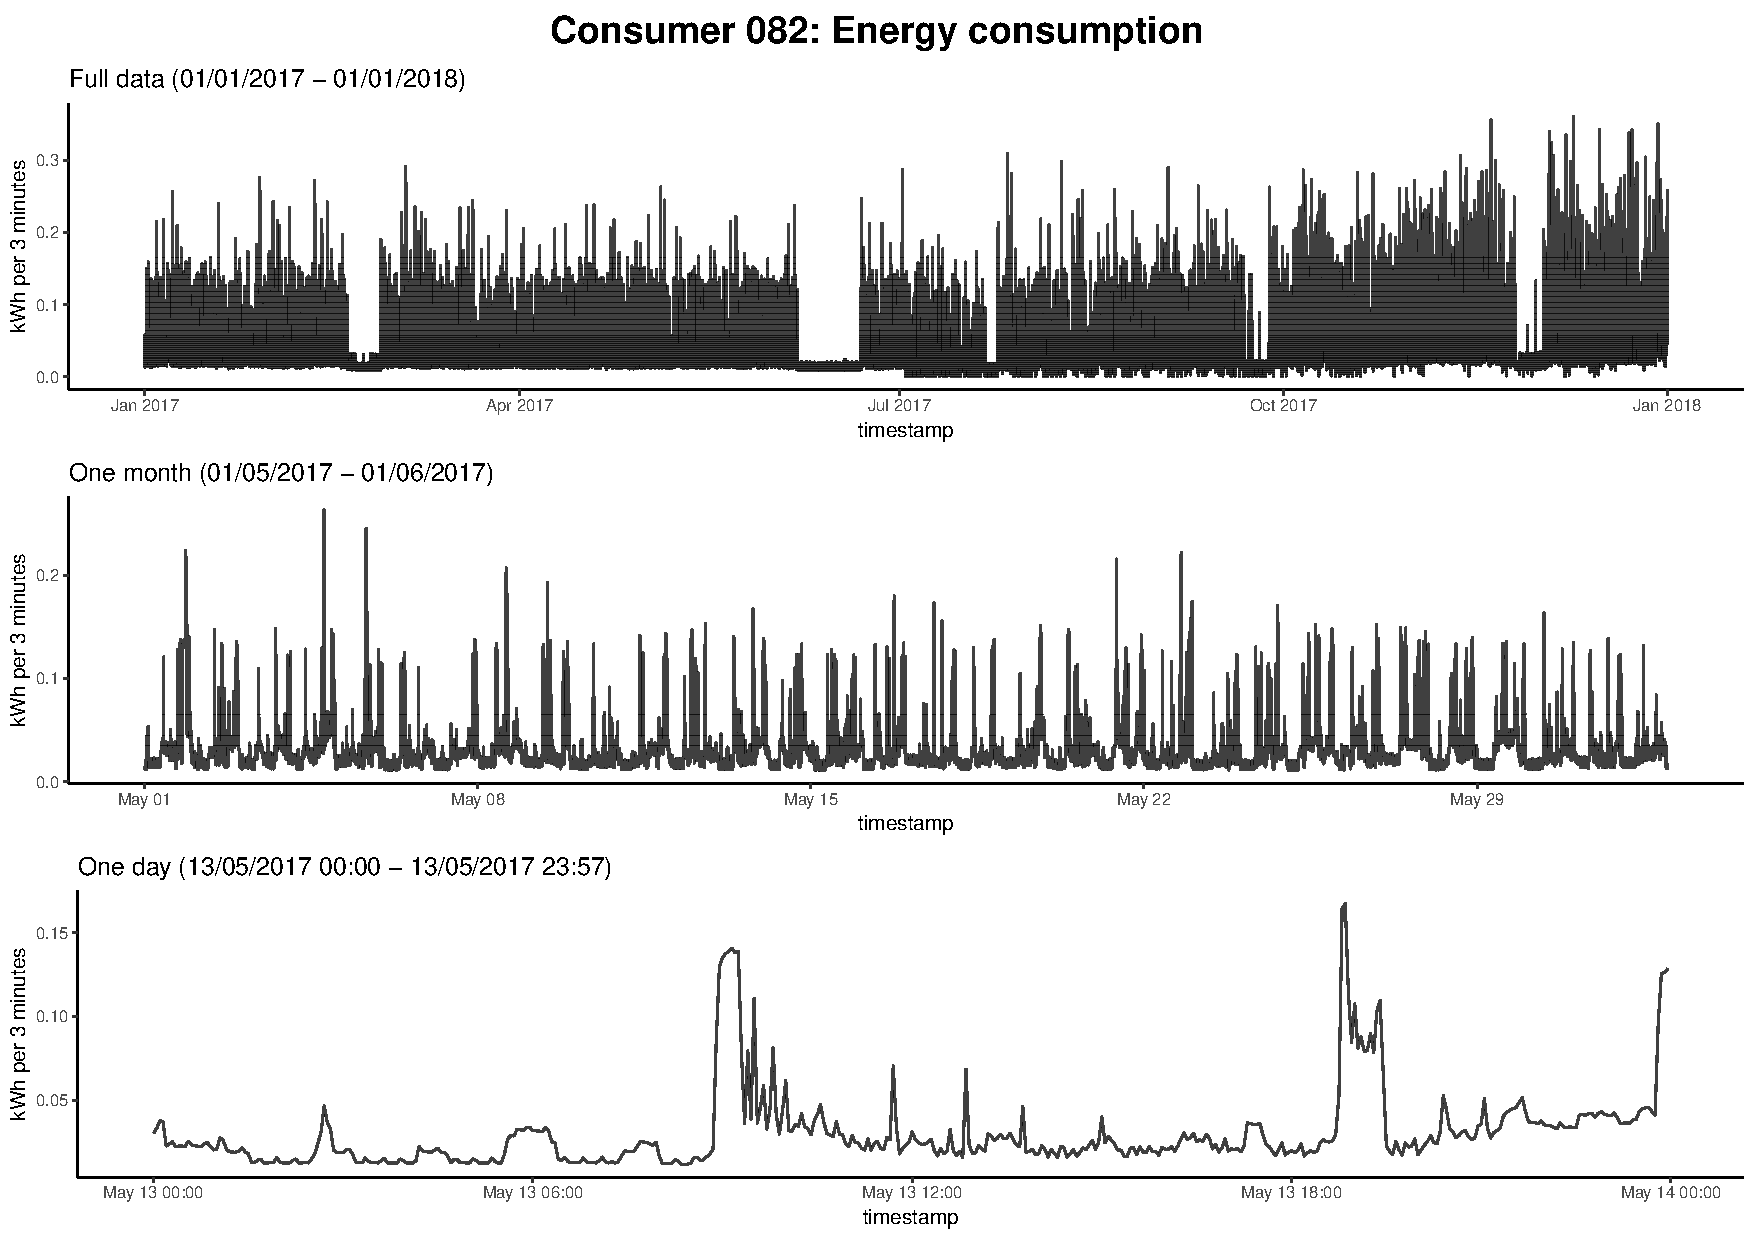
\includegraphics[width=\textwidth]{thesis/graphs/timeseries/c082_cons.pdf}
\caption[Energy consumption recordings of consumer 082]{Energy consumption recordings of consumer 082. The first panel shows the full year 2017, the second panel zooms in to one month (May), and the third panel zooms in to one day (May, 13). \quantnet\href{https://github.com/QuantLet/BLEM/tree/master/BLEMplotEnergyData}{BLEMplotEnergyData}}
\label{Fig:energycons_c082}
\end{figure}

Notably, there are two extended (in March and June) and three shorter periods (in July, September, and December) of clearly distinguishable low consumption and low fluctuation levels. The most likely explanations for these low, stable energy consumption periods are holidays, in which the household members are on vacation and leave appliances that are on standby or always turned on as the only energy consumers. This exemplifies the fact, that household members' behaviour is the biggest driver of fluctuations in the energy consumption of a household and the almost only cause for uncertainty in the time series.

Interestingly, the consumption time series of consumer 082 shows an increase in mean consumption starting with October 2017. This could be explained by colder outside temperatures. However, within the first quarter of 2017, no equivalent decrease in the mean energy consumption can be seen. Therefore, the reason for this increase might be given by newly acquired household appliances which are increasingly used with the approaching winter as the household members spend more time indoors.

The second panel zooms to just one month making daily fluctuation patterns already visible. In May there seem to be no abnormal consumption patterns. There are a few peaks in the first and third week of May that stand out, but no longer periods of very low energy consumption. More interestingly seems to be the last panel, which zooms in to just one day of energy consumption, i.e. May 13, 2017. This day was chosen for no particular reason other than that it is more or less in the middle of the month shown in the second panel. May 13, however, nicely exemplifies a usual pattern of energy consumption: There is low and rather stable energy consumption from midnight until about 7.30 a.m. which only fluctuates in a systematic and repeated way. Most probably, this ``base consumption" is caused by appliances in standby and ``always on" appliances, such as a fridge and/or freezer. At around 7.30 a.m., the household members probably wake up and the energy consumption spikes for the next 30 minutes -- the light is turned on, coffee is made, the stove is turned on, and maybe a flow heater is used to shower with hot water. As the household members leave the house (May 13 is a Monday), the consumption slowly decreases again. In the evening at about 6.30 p.m. energy consumption spikes again, probably caused by dinner preparations (and the usage of a microwave or stove). Not intuitively explainable, however, is the spike which is visible just before midnight. This spike, again, highlights the extreme uncertainty contained in individual household energy consumption. It is mostly caused by human behavior, which can seem quite erratic by just looking at energy consumption patterns without context.

To get a better impression of the representativity of consumer 082's energy consumption, it is compared to the other data sets available for this study. Figure~\ref{Fig:cons_total_consumption} shows the total energy consumption 2017 in kWh of all consumers. As can be seen, consumer 082 (labelled c082 in Figure~\ref{Fig:cons_total_consumption}) is at the lower end of the top quartile of the total energy consumption distribution across all consumers. The household's total energy consumption in 2017 was 6752.763 kWh. According to \citet{Stromspiegel:2017}, this number corresponds to a category D five-person household (on a scale from A (very low) to G (very high energy consumption)) that is heating its water with electricity. That means, the household of consumer 082 is either very big or has a comparatively very high energy consumption. Consumer 067, on the contrary, is remarkable as total consumption here is with only 40 kWh quite close to zero. At the high end of total consumption is consumers 025 with almost five times the total consumption of the average consumer in this data sets. Summary statistics for the total energy consumption of consumer households in 2017 can be found in Appendix~\hyperlink{AppB1:Tables:totalcons}{B1}.

\begin{figure}[htbp]
 \centering
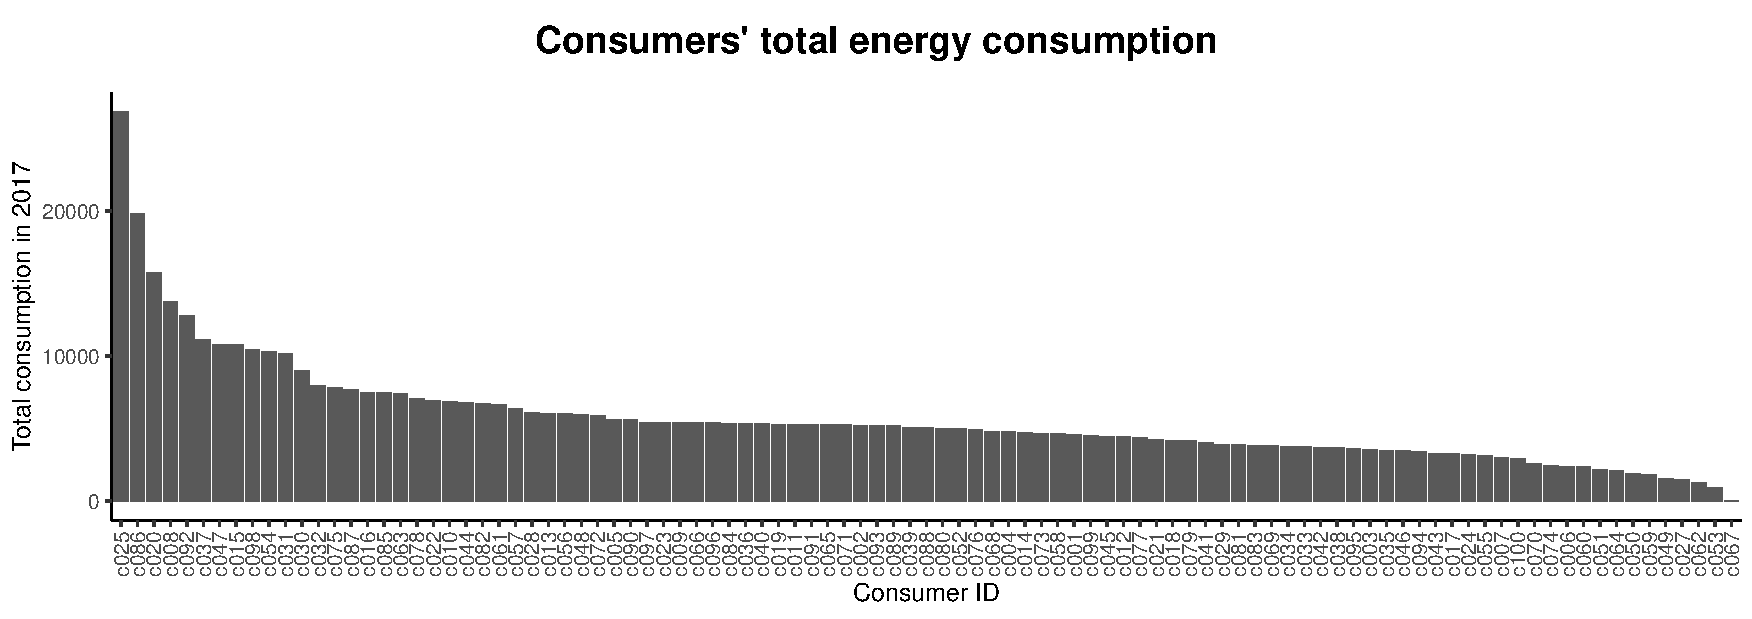
\includegraphics[width=\textwidth]{thesis/graphs/consumer_totalconsumption2.pdf}
\caption[Consumers' total energy consumption (in kWh) in 2017]{Consumers' total energy consumption (in kWh) in 2017 ordered from high to low. \quantnet\href{https://github.com/QuantLet/BLEM/tree/master/BLEMdescStatEnergyData}{BLEMdescStatEnergyData}}
\label{Fig:cons_total_consumption}
\end{figure}

Figure~\ref{Fig:cons_boxplots_consumption} offers another perspective on the consumers' energy consumption. The figure shows a boxplot for each consumer's distribution of energy consumption per 3-minute interval. That means, the median line in the boxplot of a consumer is the consumers median consumption per 3-minute interval, while the box encloses the interquartile range (IQR) of the 3-minute consumption values of this particular consumer. It is apparent, that the IQR is for almost all consumers relatively small compared to the total range of their consumption values. All points plotted above the boxplots' whiskers are consumption values greater than the third quartile plus 1.5 $\times$ IQR. This again shows that there is a substantial amount of extreme values -- for which the description ``outlier" not necessarily fits as they obviously occur quite often -- which are, most likely, hard to predict with standard forecasting methods.

\begin{figure}[htbp]
 \centering
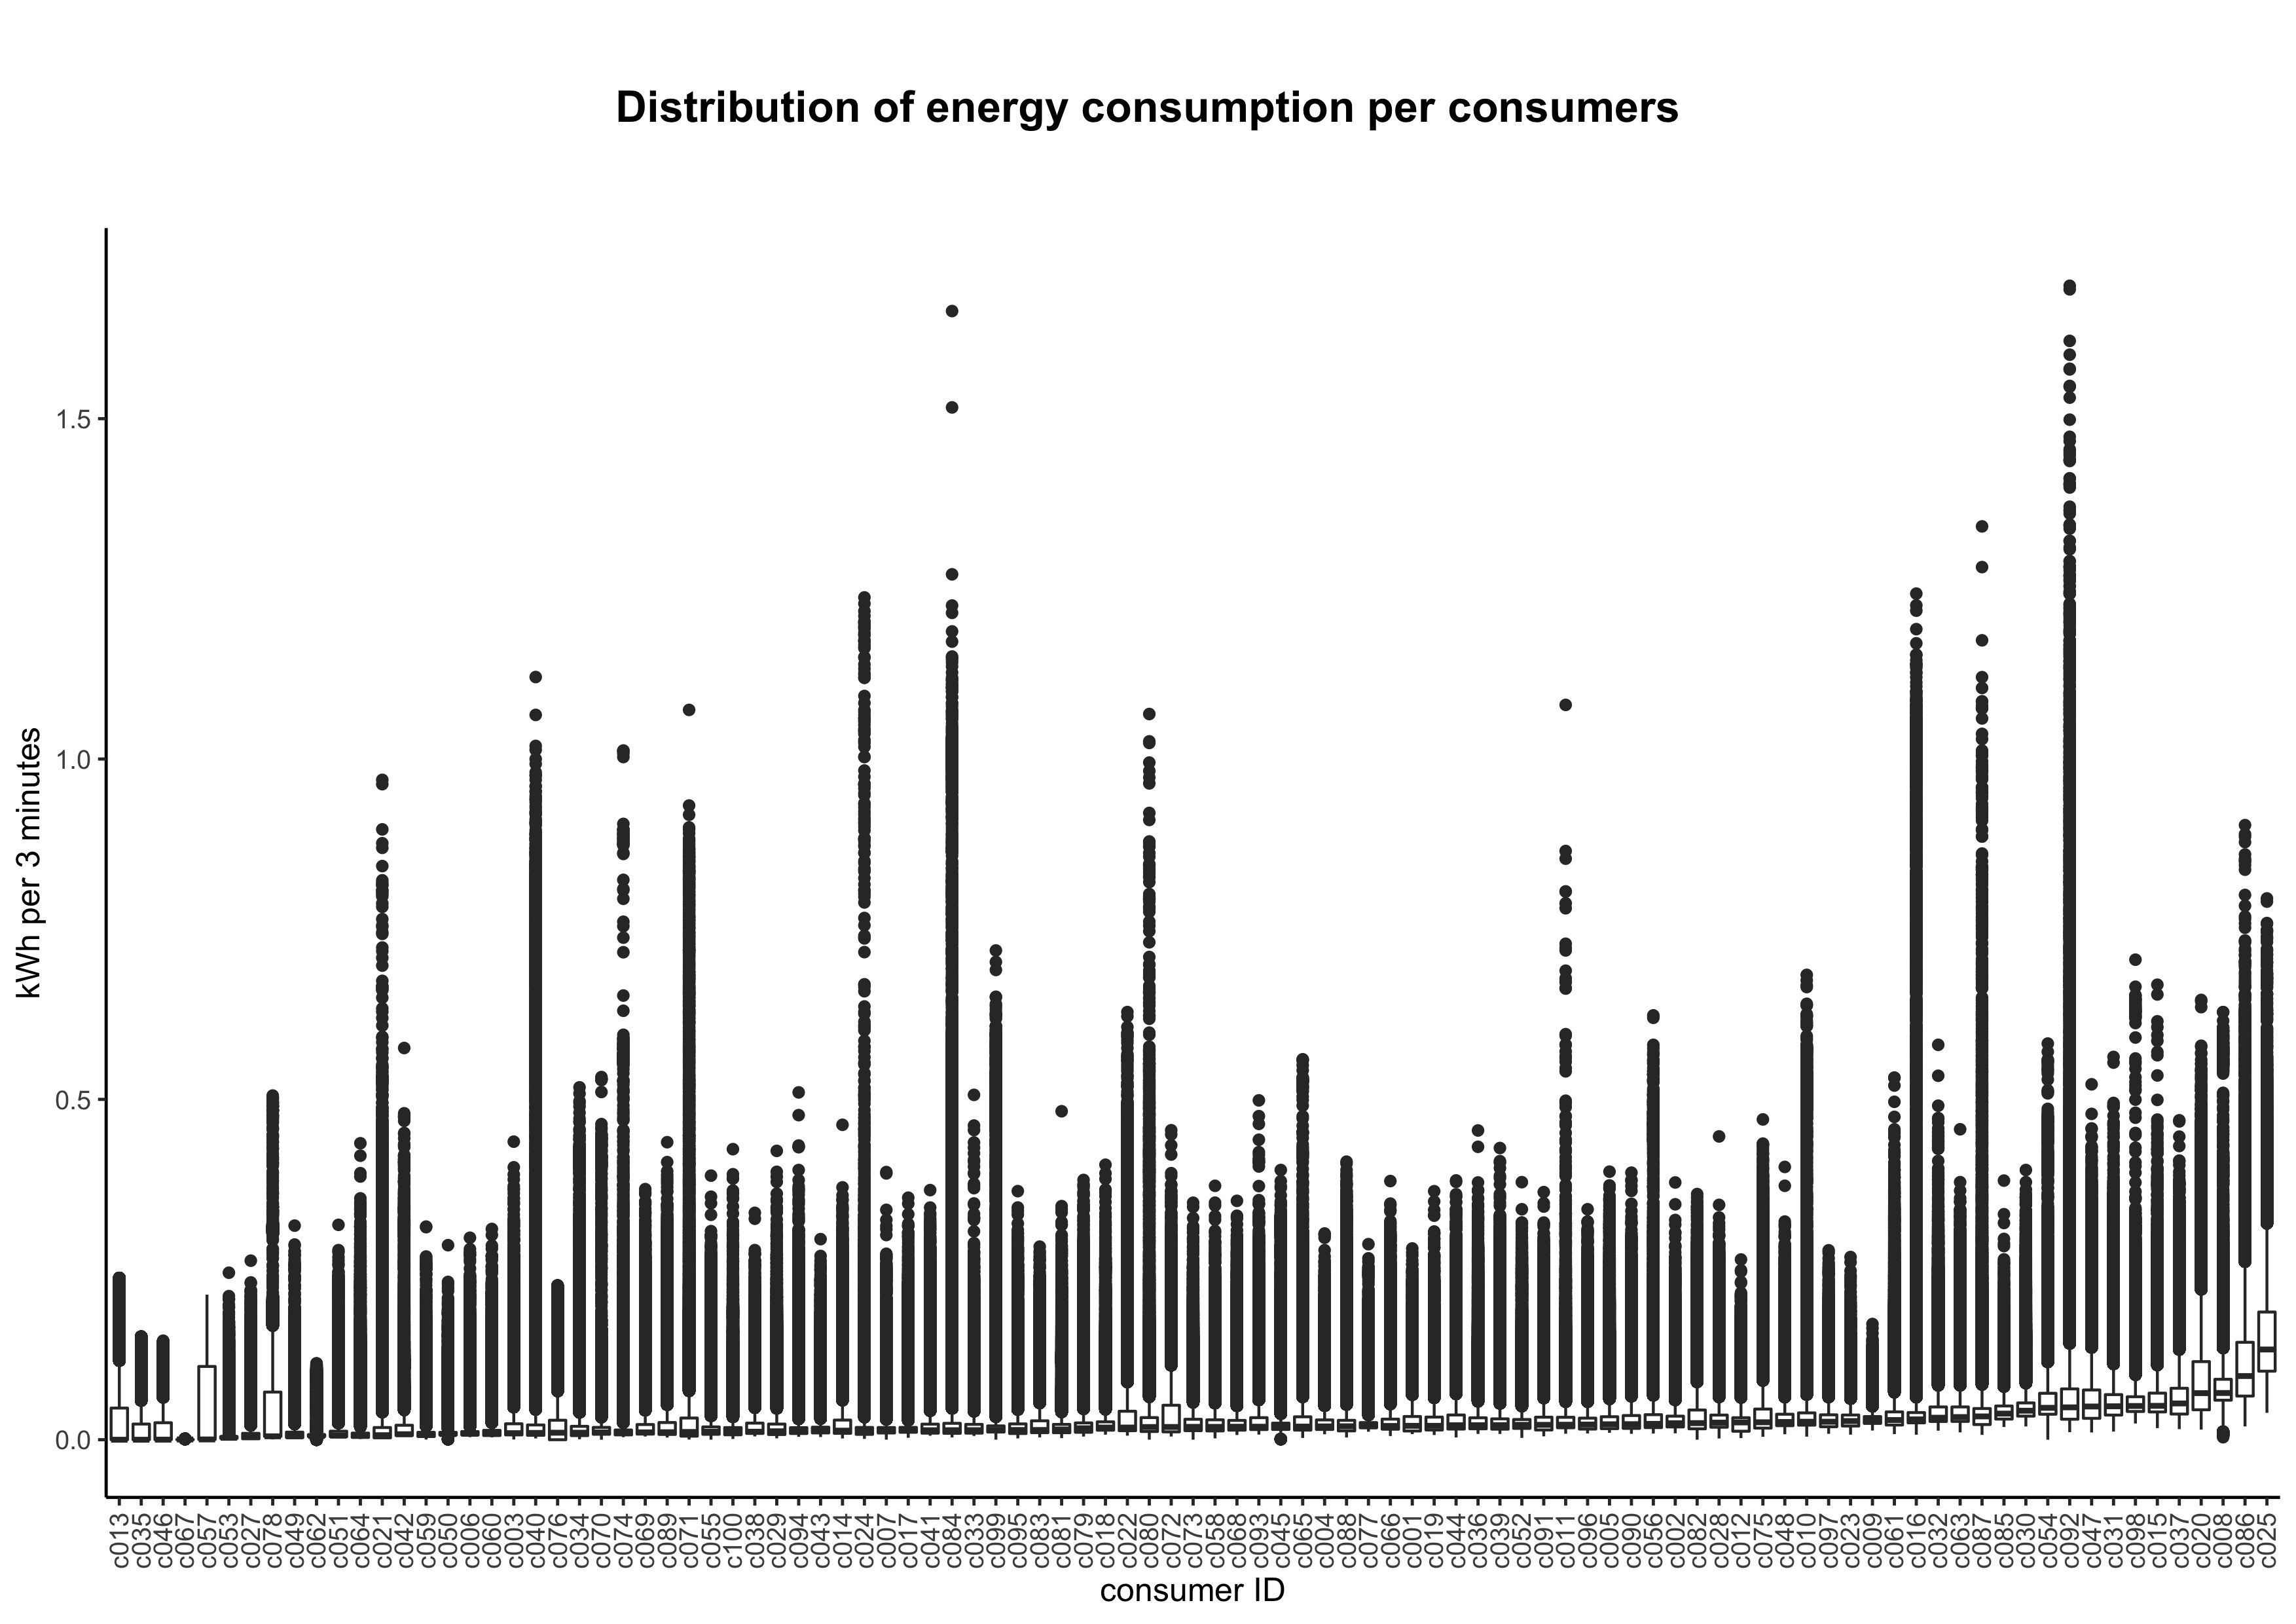
\includegraphics[width=\textwidth]{thesis/graphs/consumer_boxplots_consumption.jpg}
\caption[Boxplots of each consumer's energy consumption in kWh per 3-minute interval]{Boxplots of each consumer's energy consumption in kWh per 3-minute interval. \quantnet\href{https://github.com/QuantLet/BLEM/tree/master/BLEMdescStatEnergyData}{BLEMdescStatEnergyData}}
\label{Fig:cons_boxplots_consumption}
\end{figure}

%%%%%%%%%%%
\subsubsection{Prosumer data sets}

As it turns out, the prosumer data sets show very different consumption patterns than pure consumers. This may be due to the fact, that the recorded energy consumption per 3-minute interval is the net value of the actual energy consumption and the energy production in the same interval. For example, if prosumer 024's recorded consumption value is 0.021 kWh in the time period from 2017-05-13 06:03:00 to 06:06:00, and its energy production in the same interval is 0.018 kWh (which is not recorded and therefore not known), its actual energy consumption in that time interval is 0.039 kWh. However, this actual energy consumption is unknown as the energy production per 3-minute interval is not recorded. Only a surplus of energy production over consumption would be recorded as an increase in the energy out readings (see Table~\ref{Tab:p089}) -- which is not the case in this example.

Visual inspection of the consumption time series of the prosumer data sets already reveals that the consumption patterns in most cases do not resemble the consumer households' consumption patterns. Generalized, four types of consumption patterns can be found in the prosumer data: (1) The net energy consumption of the prosumer is zero at night, starts to increase at around 6 a.m., fluctuates over daytime, and decreases to zero again at around 6 p.m. (see exemplary prosumer 004 in Figure~\ref{Fig:prosenergycons_peculiar}). (2) The net energy consumption is mostly non-zero and fluctuates (in a regular pattern) at low levels with occasional net consumption spikes (see exemplary consumer 050 in Figure~\ref{Fig:prosenergycons_peculiar}). This is the most generic type of prosumer energy consumption patterns. (3) The net consumption is for most of the year zero (see exemplary prosumer 061 in Figure~\ref{Fig:prosenergycons_peculiar}). This may be due to a surplus in net energy production. (4) The net energy consumption is mostly non-zero and fluctuates very little at a relatively high level (see exemplary prosumer 093 in Figure~\ref{Fig:prosenergycons_peculiar}). The net energy consumption drops only occasional from this high level. Type (1) and (2) represent the majority of data sets. Type (1) is very easily identifiable and represents 30~\% of the data sets. Type (2) is more generic and therefore comprises more heterogenic patterns with 56~\% of the data sets belonging to this type. Type (3) and (4), exemplary shown in the lower two panels of Figure~\ref{Fig:prosenergycons_peculiar}, only represent a minority of the data sets.

\begin{sidewaysfigure}[htbp]
    \centering
    \begin{minipage}[h]{\dimexpr.5\textheight-0.15em}
    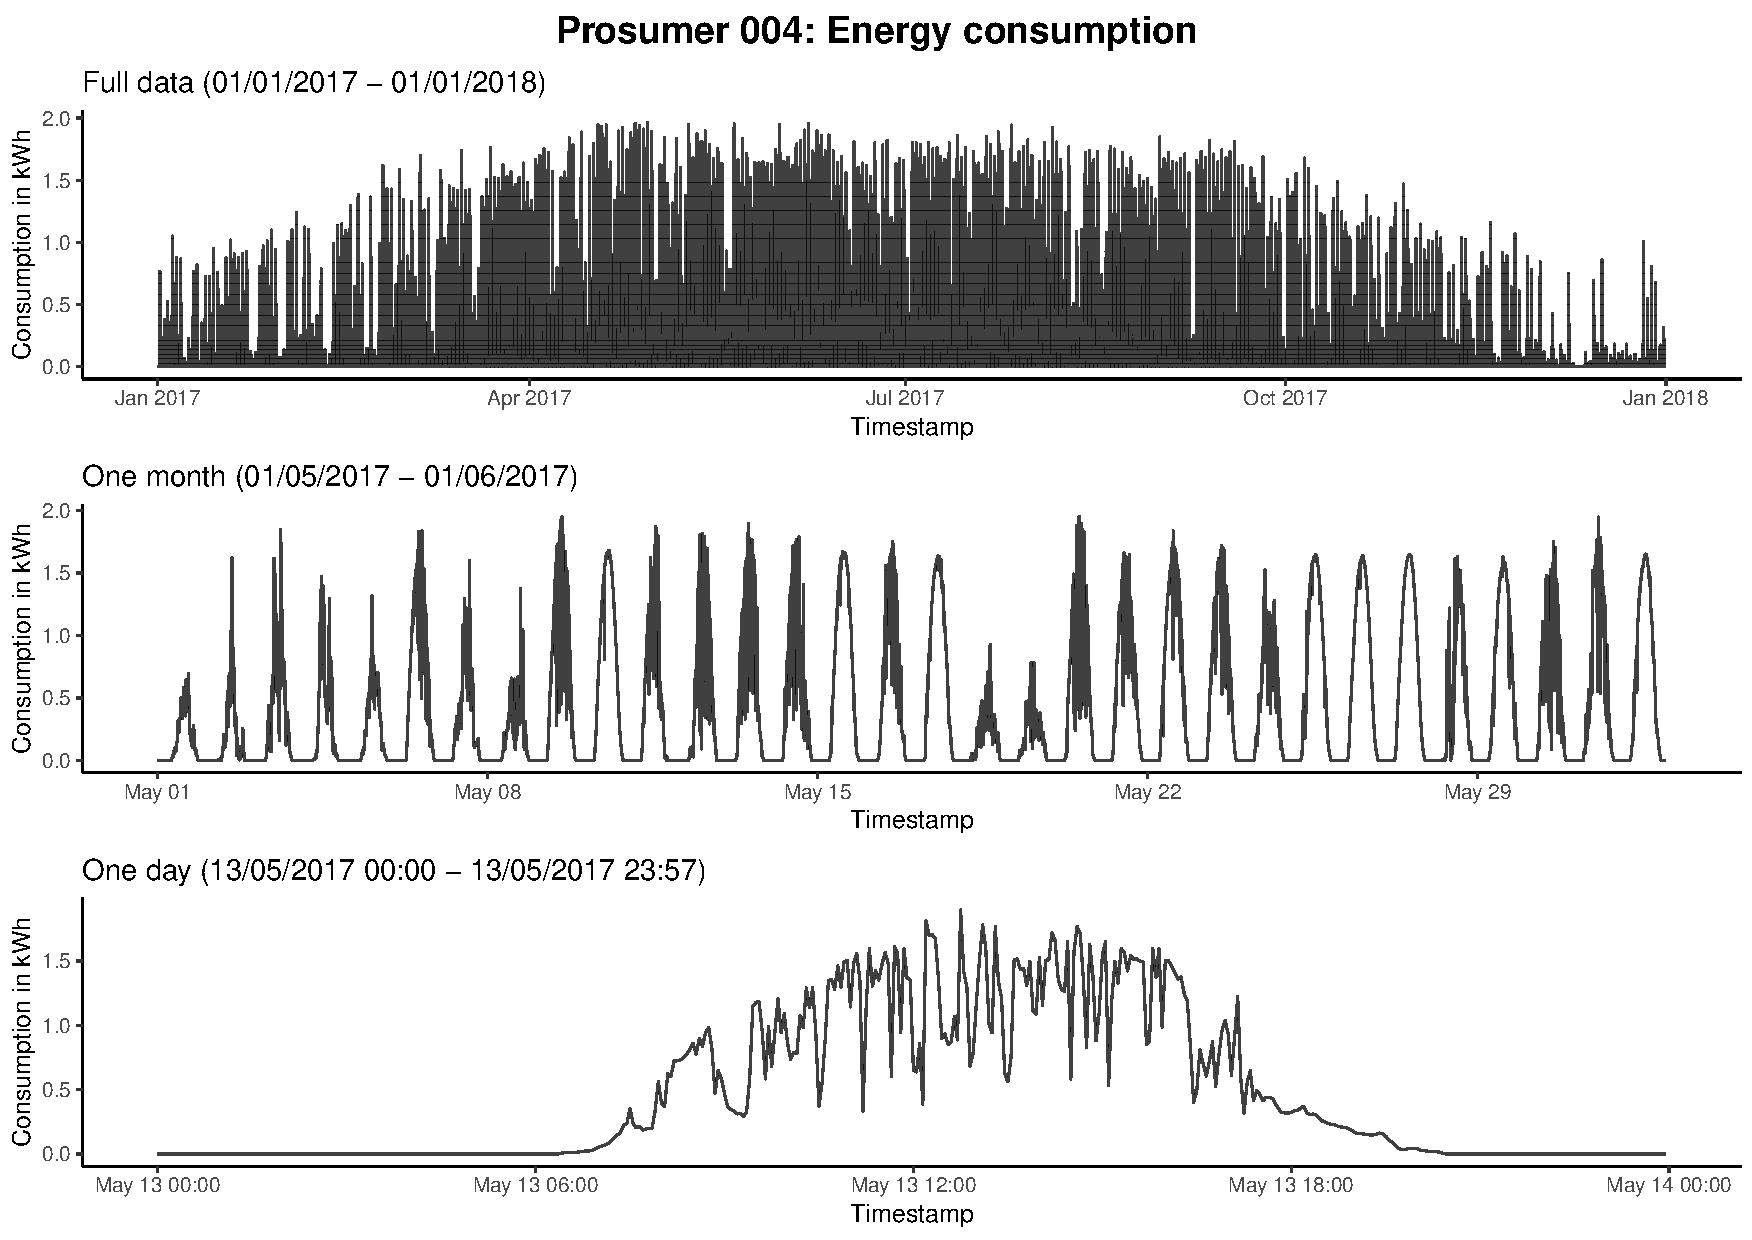
\includegraphics[width=\textwidth]{thesis/graphs/timeseries/p004_cons.pdf}
    \end{minipage}
    \begin{minipage}[h]{\dimexpr.5\textheight-0.15em}
    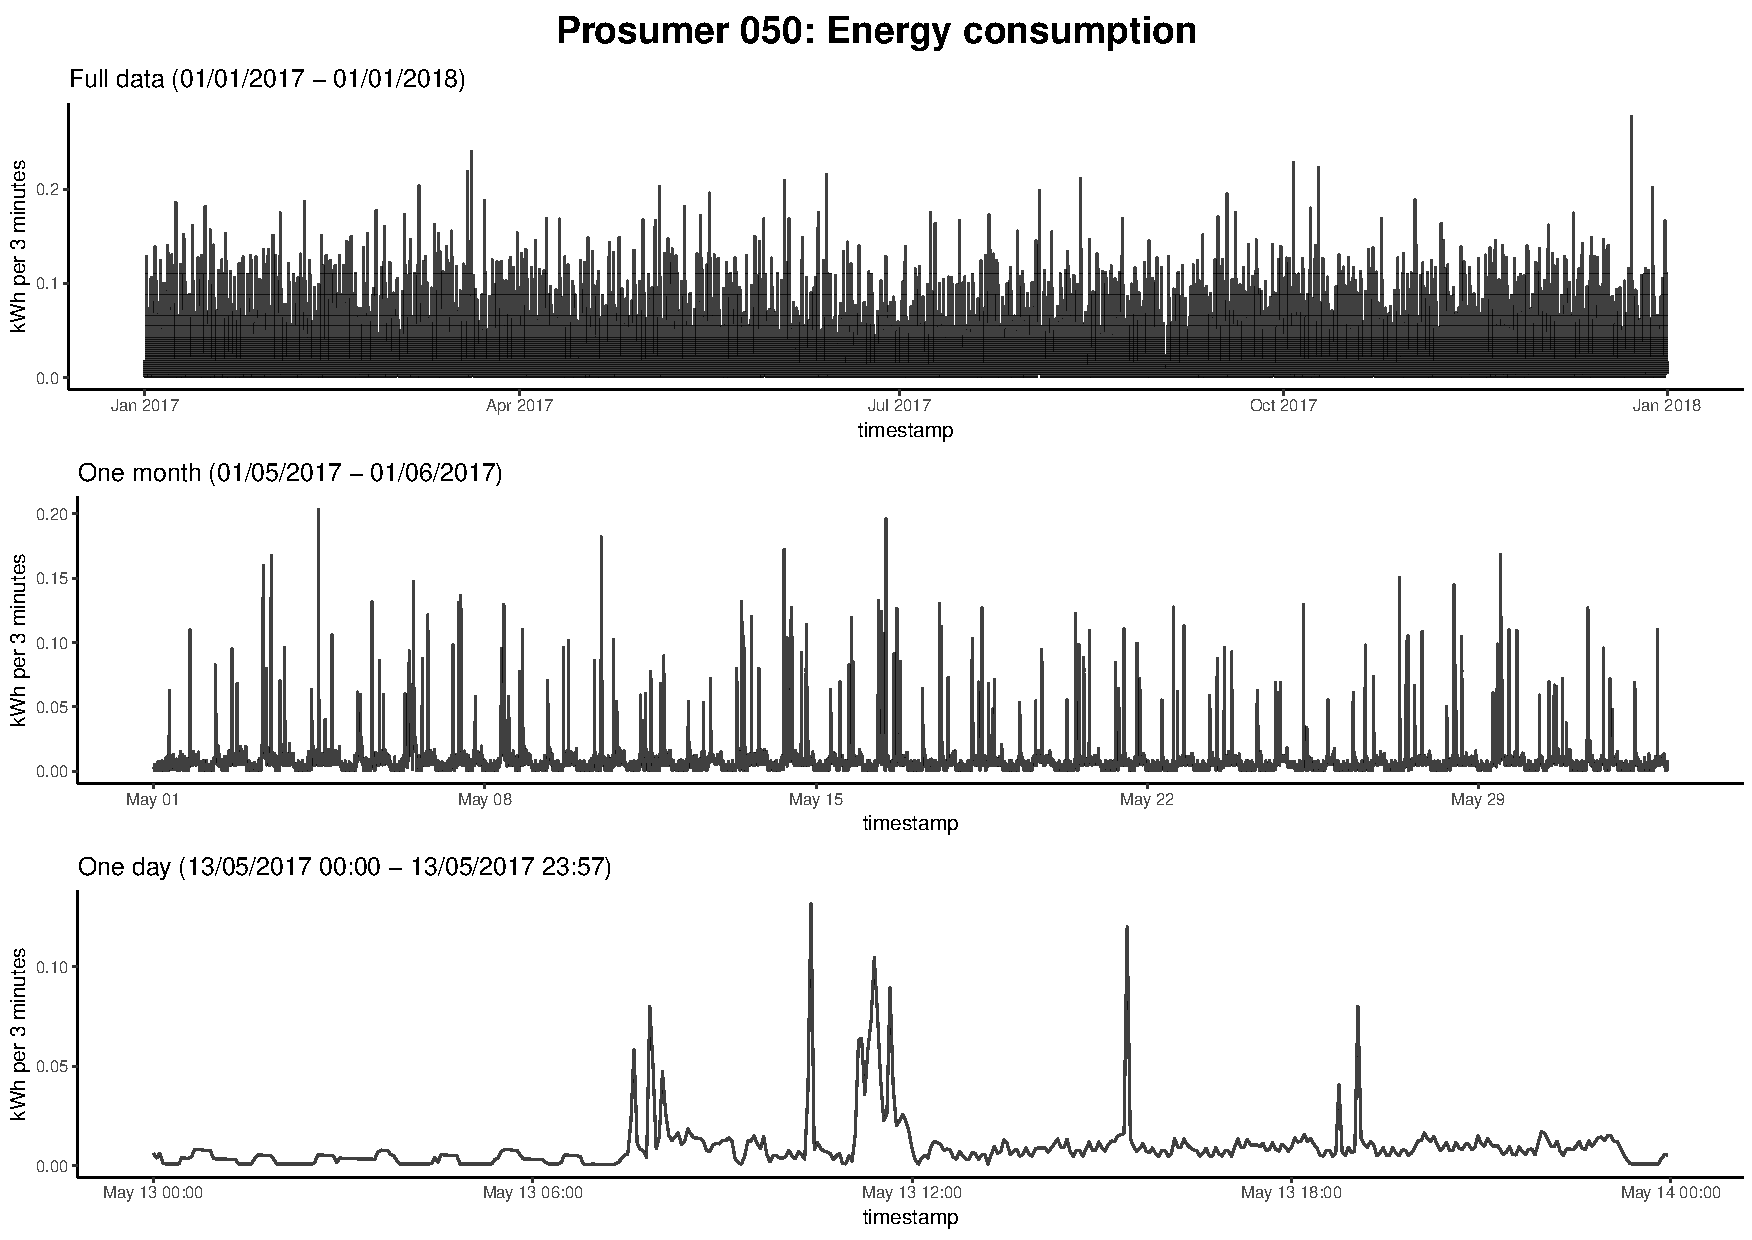
\includegraphics[width=\textwidth]{thesis/graphs/timeseries/p050_cons.pdf}
    \end{minipage}\\
    
    \begin{minipage}[h]{\dimexpr.5\textheight-0.15em}
    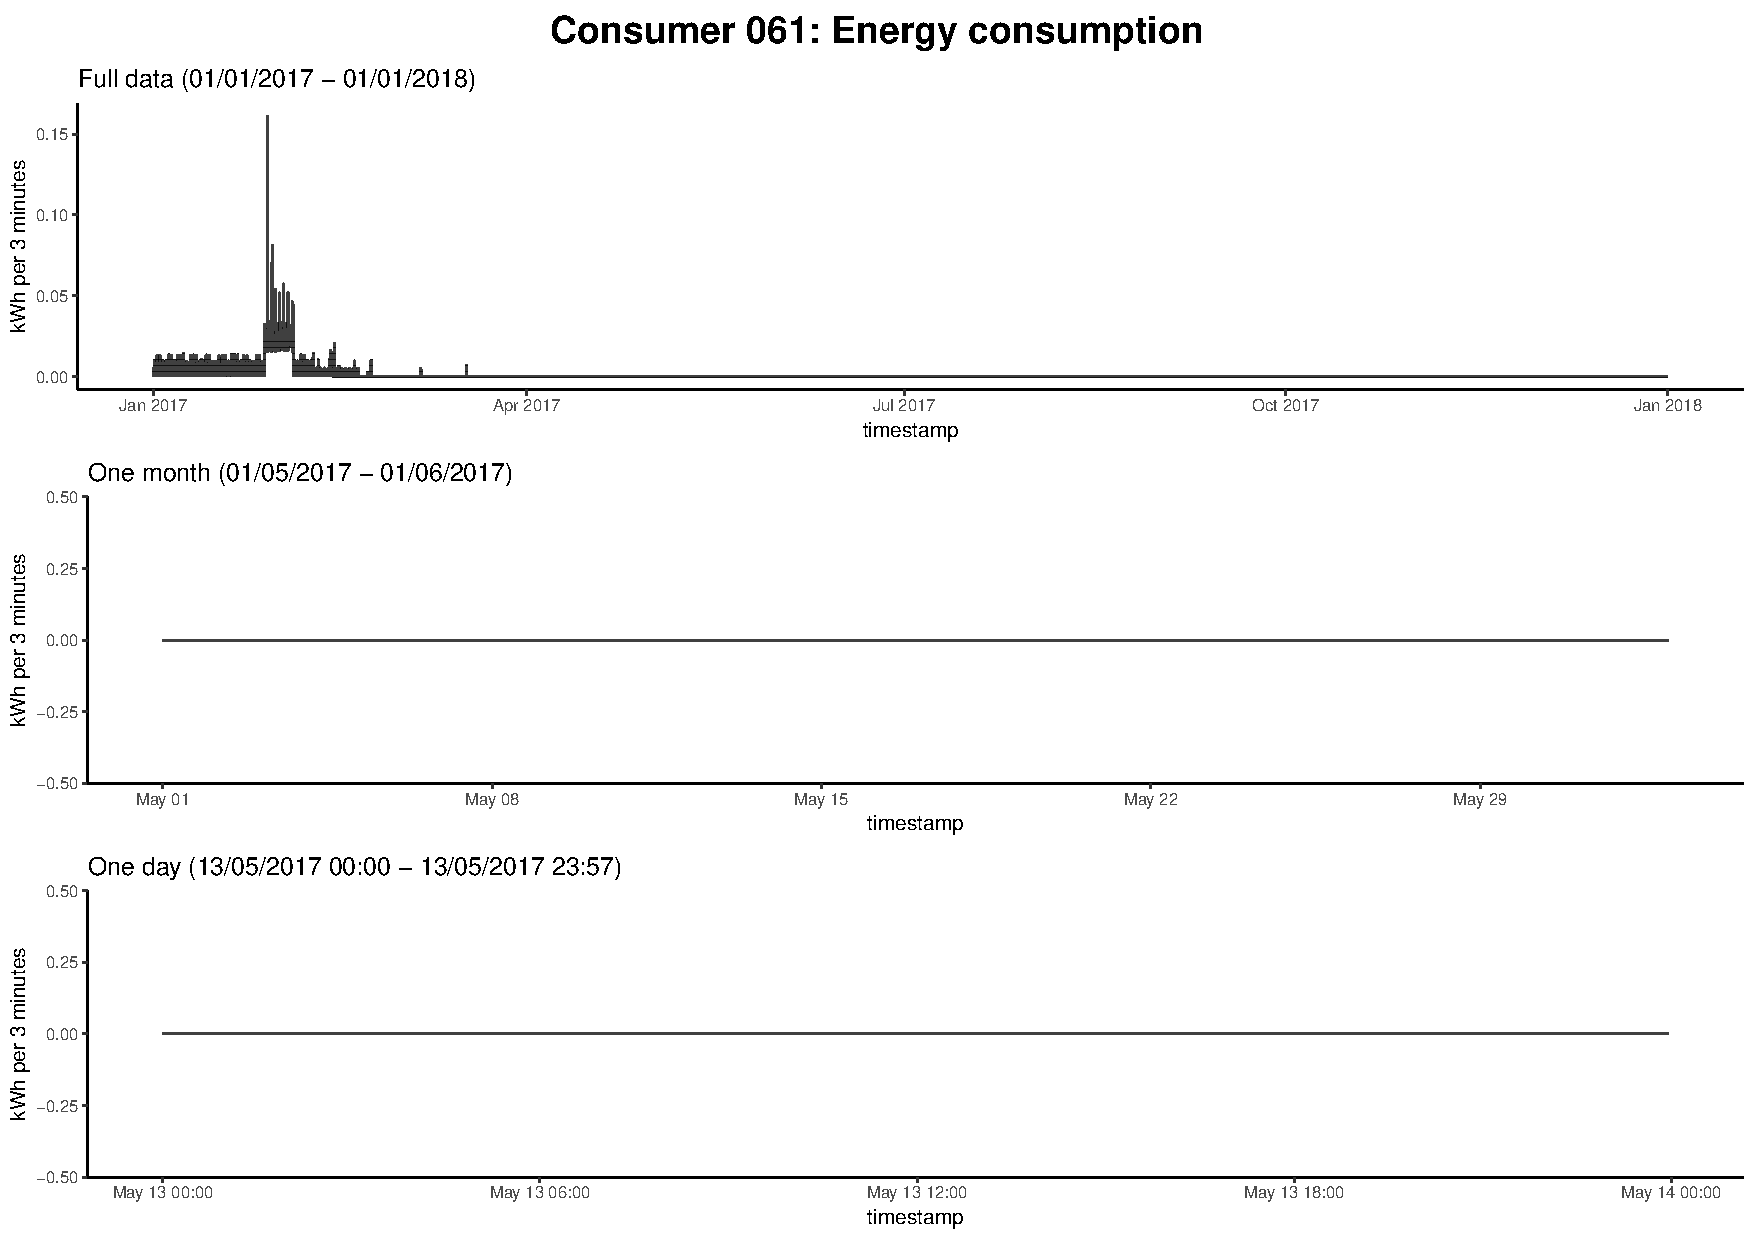
\includegraphics[width=\textwidth]{thesis/graphs/timeseries/p061_cons.pdf}
    \end{minipage}
    \begin{minipage}[h]{\dimexpr.5\textheight-0.15em}
    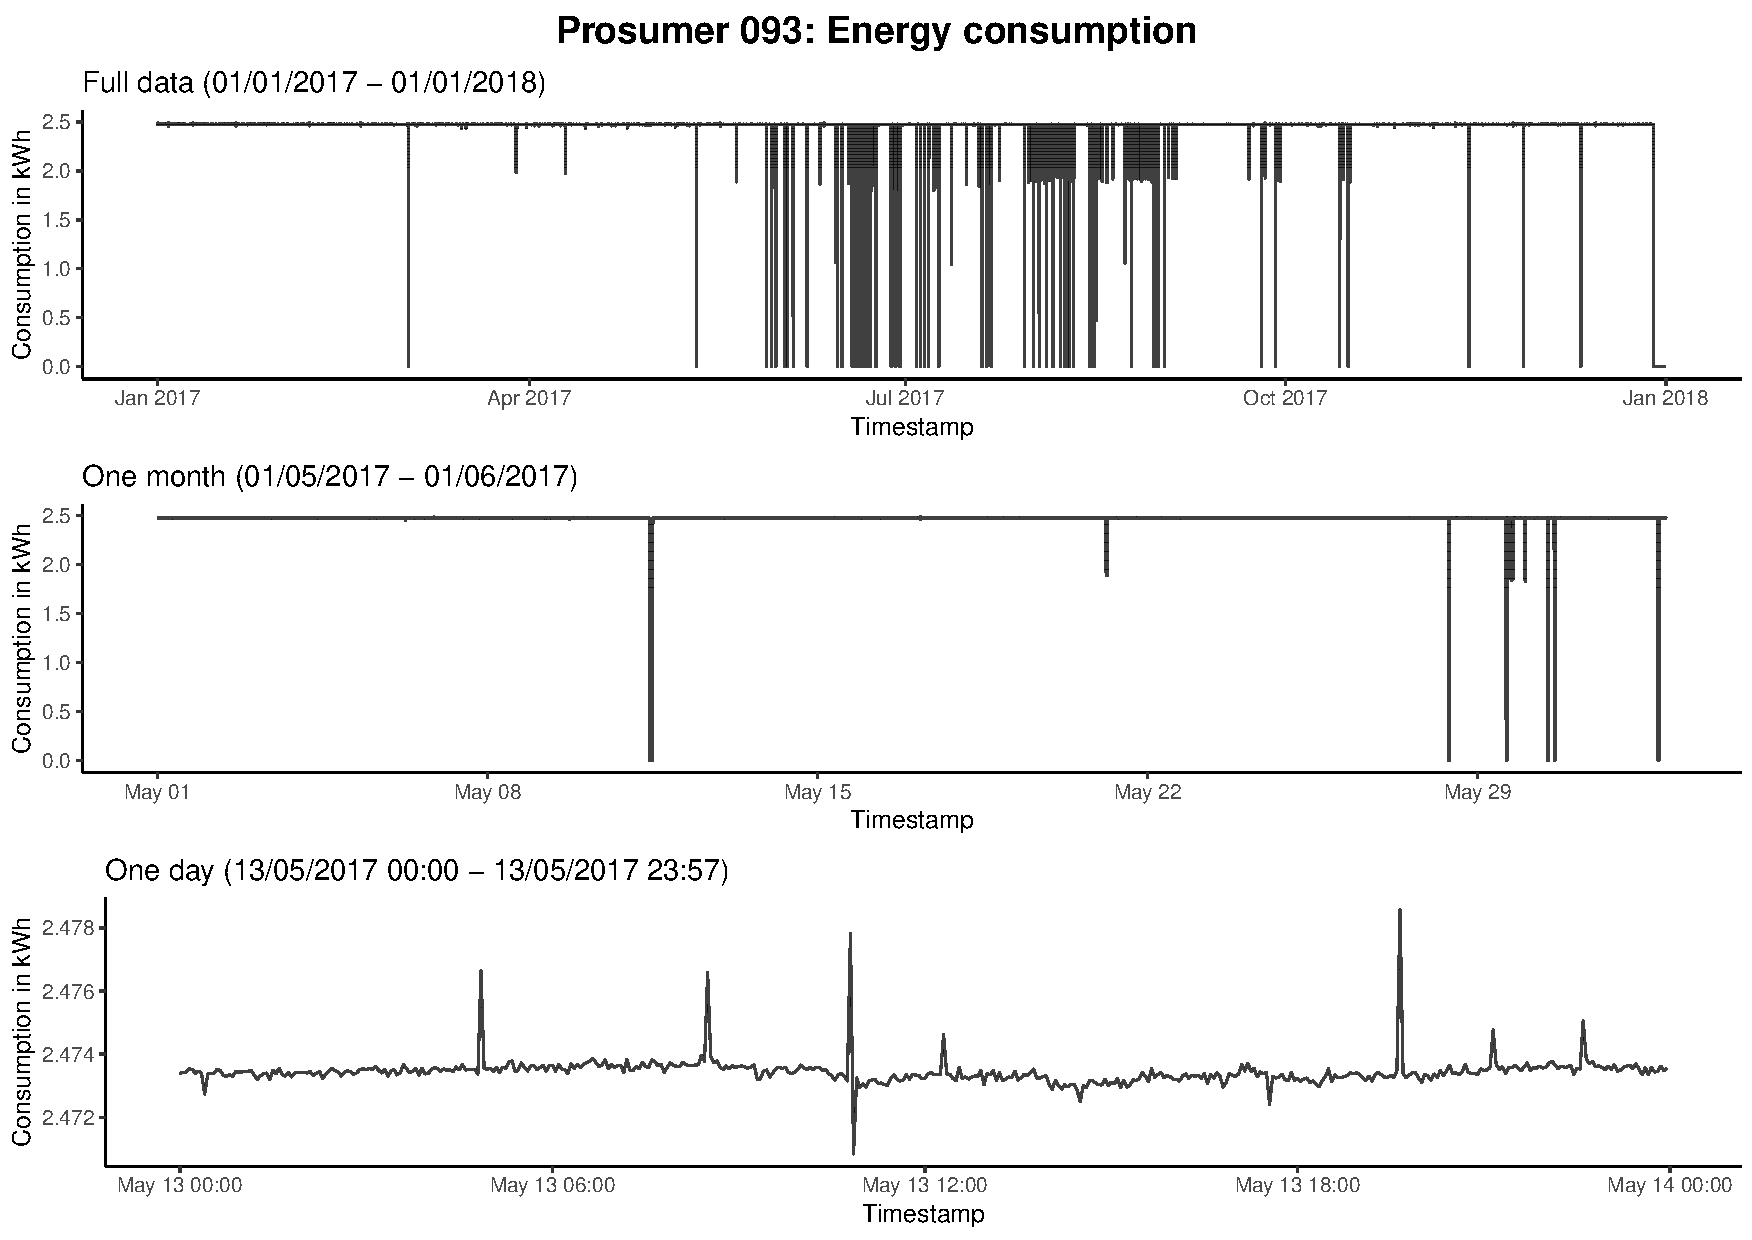
\includegraphics[width=\textwidth]{thesis/graphs/timeseries/p093_cons.pdf}
    \end{minipage}
    
    \caption[Different types of prosumer energy consumption patterns]{Different types of prosumer energy consumption patterns. \quantnet\href{https://github.com/QuantLet/BLEM/tree/master/BLEMplotEnergyData}{BLEMplotEnergyData}}
    \label{Fig:prosenergycons_peculiar}
\end{sidewaysfigure}

In conclusion, it becomes clear that the net energy consumption of prosumers may exhibit very different patterns than the energy consumption of consumers. This exacerbates the prediction task for prosumers significantly.

Furthermore, the total consumption of prosumers follows a very different distribution than the total consumption of consumers. The maximum total net consumption of a prosumer was 424,893.434 kWh, which is by a factor of 15 more than the maximum total net consumption of a prosumer. 19 out of 100 prosumers net consumed more energy than the biggest consumer household contained in the data. Also, the dispersion of the total net consumption is much higher with an IQR of 22,149 kWh for prosumers' total net consumption compared to an IQR of 2,542 kWh for consumers' total consumption in 2017.

\begin{figure}[htbp]
 \centering
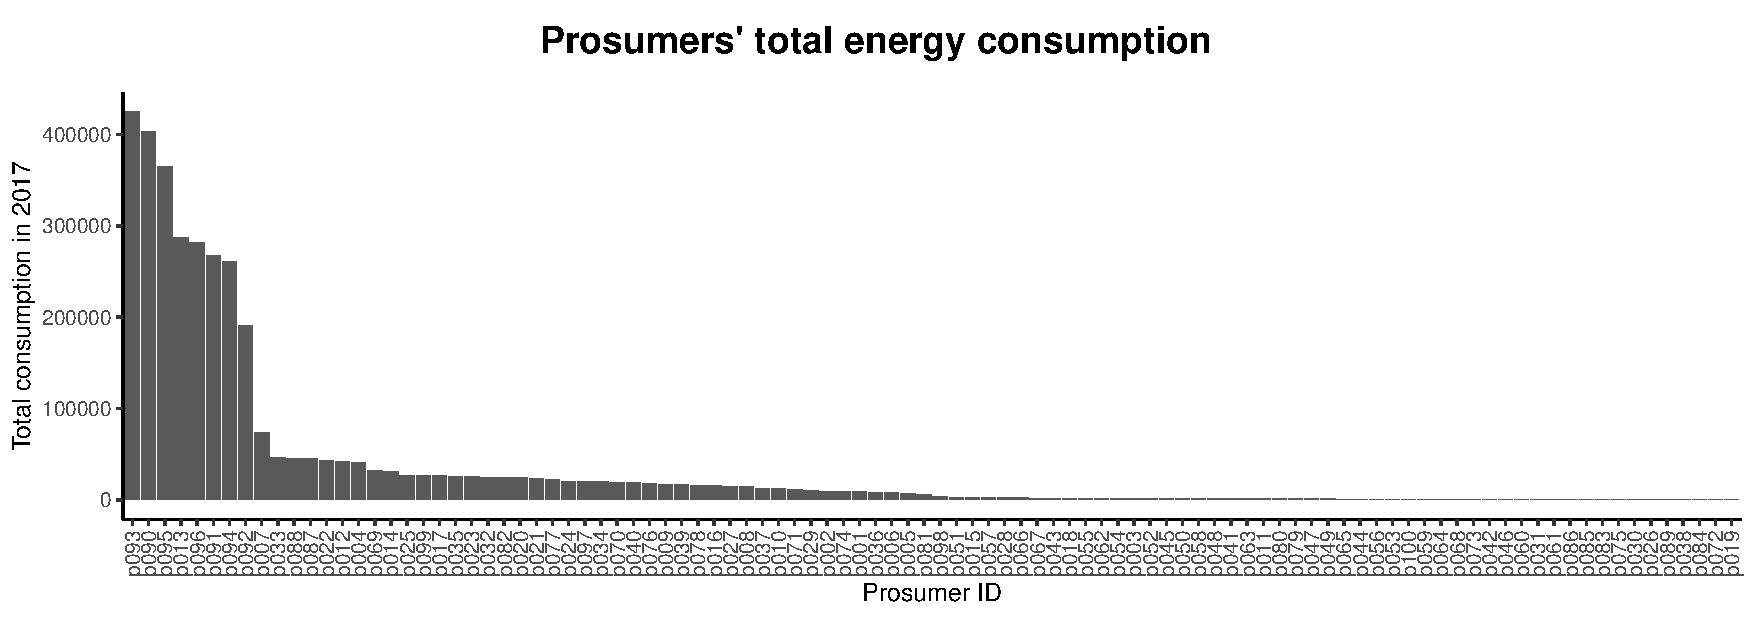
\includegraphics[width=\textwidth]{thesis/graphs/prosumer_totalconsumption2.pdf}
\caption[Prosumers’ total energy consumption (in kWh) in 2017]{Prosumers’ total energy consumption (in kWh) in 2017 ordered from high to low. \quantnet\href{https://github.com/QuantLet/BLEM/tree/master/BLEMdescStatEnergyData}{BLEMdescStatEnergyData}}
\label{Fig:pros_total_consumption}
\end{figure}

Finally, Figure~\ref{Fig:pros_boxplots_consumption} offers another perspective on the heterogeneity of the prosumer data sets. The figure shows a boxplot for each prosumer's distribution of energy consumption per 3-minute interval. The prosumers are sorted on the x-Axis by their median net energy consumption. As can be seen, while the median for the majority of the prosumers is relatively close to zero, the IQR and the total range of net consumption values differs substantially between prosumers. Approximately the same range of net consumption values per 3-minute interval can be accompanied by a median of 0.0003 kWh (see p088 in Figure~\ref{Fig:pros_boxplots_consumption}) or by a median of 1.9110 kWh (see p094 in Figure~\ref{Fig:pros_boxplots_consumption}).

\begin{figure}[htbp]
 \centering
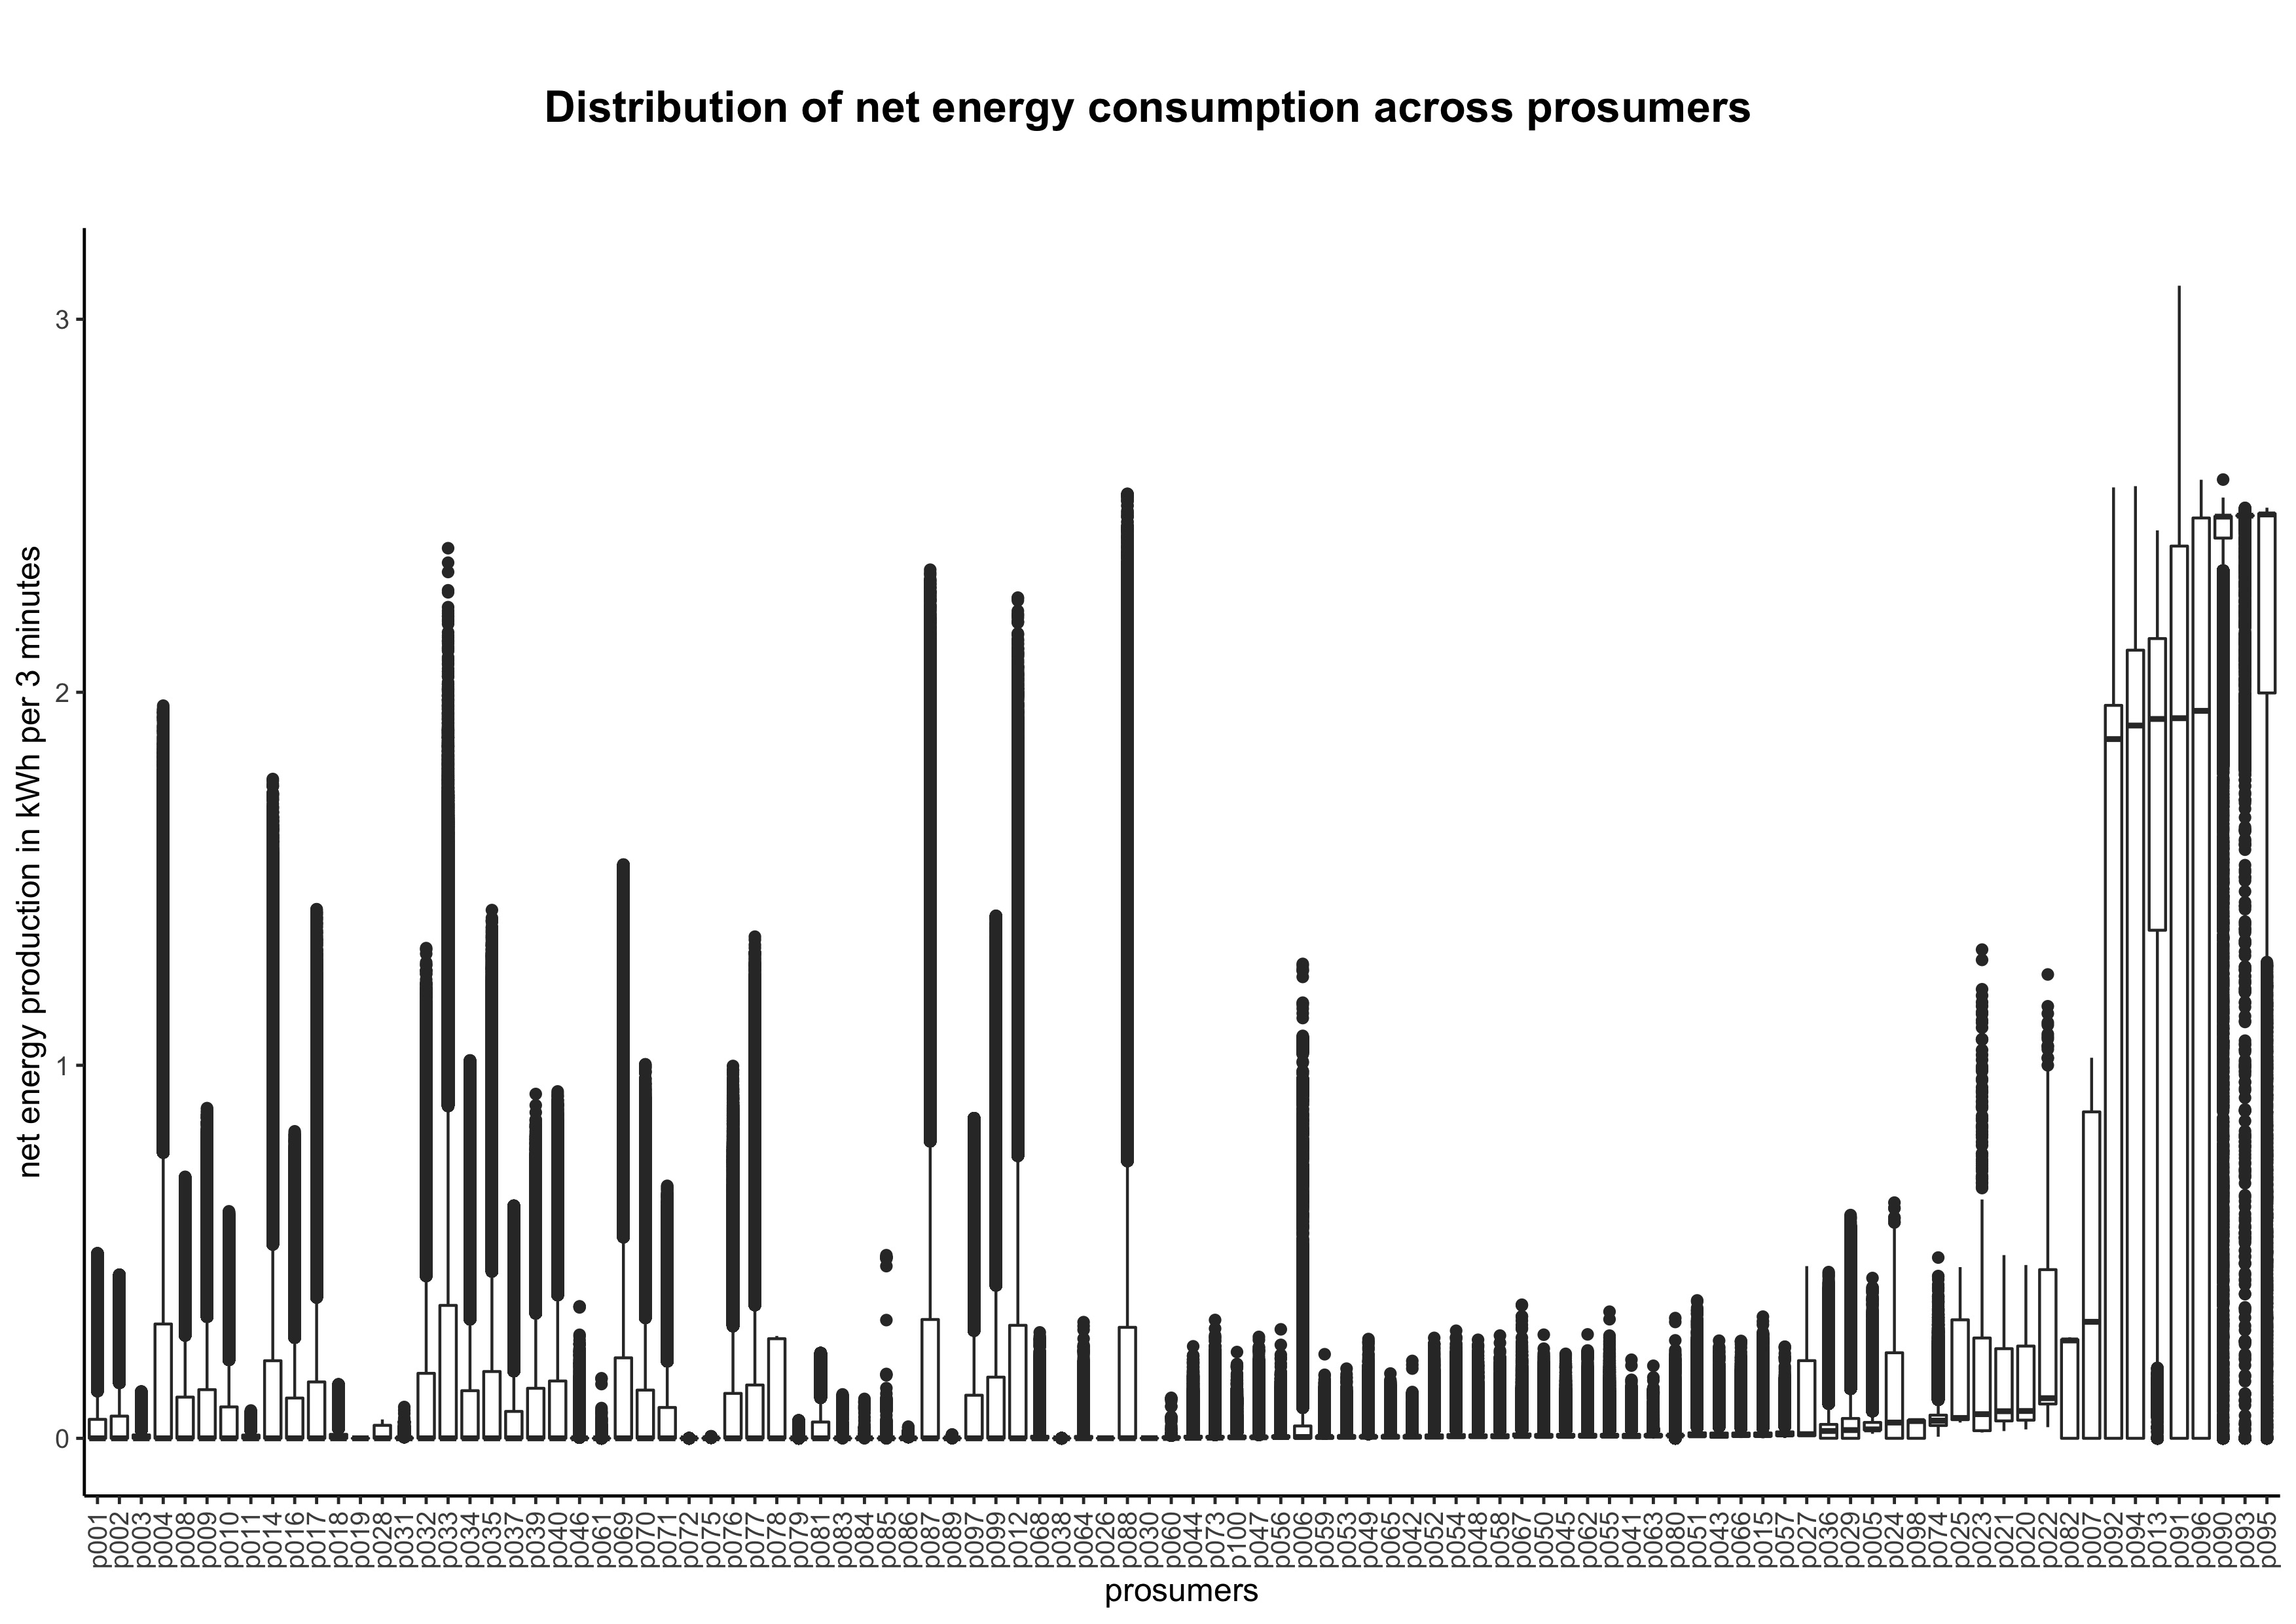
\includegraphics[width=\textwidth]{thesis/graphs/prosumer_boxplots_consumption.jpg}
\caption[Boxplots of each prosumer's net energy consumption in kWh per 3-minute interval]{Boxplots of each prosumer's net energy consumption in kWh per 3-minute interval. \quantnet\href{https://github.com/QuantLet/BLEM/tree/master/BLEMdescStatEnergyData}{BLEMdescStatEnergyData}}
\label{Fig:pros_boxplots_consumption}
\end{figure}

Prosumers are defined by the fact, that they not only consume energy but also produce energy -- primarily for their own consumption. However, any surplus in energy production over energy consumption is fed into the grid and, thus, recorded by the smart meter as an increase in the energy out readings. As explained above, these energy out readings are used to compute the net energy production per 3-minute interval by first-differencing. Surprisingly, only 14 out of 100 available prosumer data sets contained non-zero net energy production values at all. This becomes clear when looking at Figure~\ref{Fig:pros_total_production}, which shows the total net energy production of all prosumers. 86 of those prosumers fed zero kWh into the grid during 2017. The top three net energy producing prosumers, however, fed a total of 1,259,686 kWh into the grid, which is more than twice the amount all 100 consumer households consumed together\footnote{Cumulatively, the 100 consumer households, for which data is available, consumed 559,369 kWh in 2017}. For comparison, a typical photovoltaic (PV) installation on a private residential building with a roof surface area of 150 m$^2$ produces approximately 20,000 kWh per year \citep{energieatlas:2018}.

\begin{figure}[htbp]
 \centering
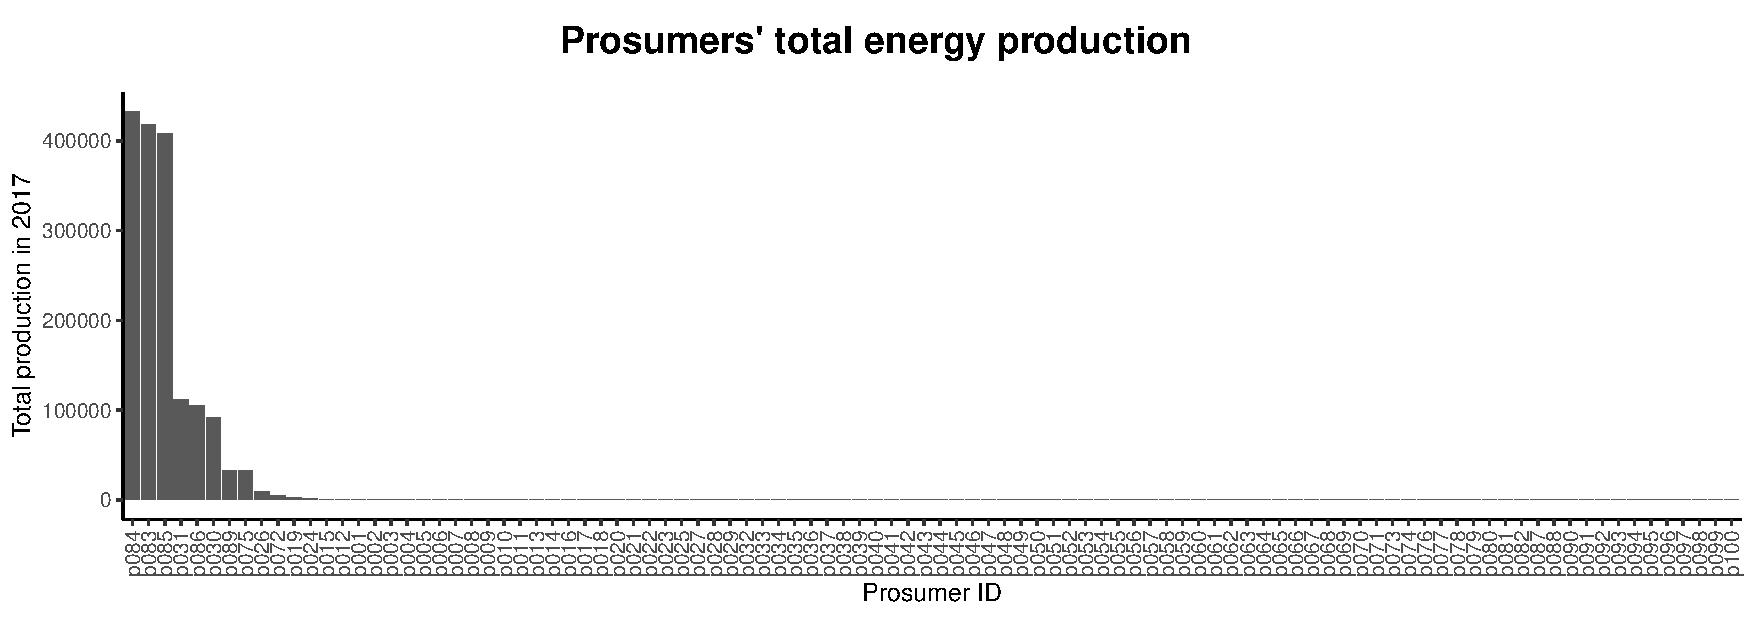
\includegraphics[width=\textwidth]{thesis/graphs/prosumer_totalproduction2.pdf}
\caption[Prosumers’ total energy production (in kWh) in 2017]{Prosumers’ total energy production (in kWh) in 2017 ordered from high to low. \quantnet\href{https://github.com/QuantLet/BLEM/tree/master/BLEMdescStatEnergyData}{BLEMdescStatEnergyData}}
\label{Fig:pros_total_production}
\end{figure}

Prosumer 026, for example, has a relatively low total net energy production. However, its net energy production pattern looks like a typical household with a PV installation (see Figure~\ref{Fig:energyconsprod_p026p086}). The net energy consumption is (almost) always zero, while the net energy production on most days rather smoothly increases and decreases throughout the day with occasional drops, probably caused by changes in the cloud cover. Furthermore, the net energy production increases in the summer months and decreases notably in winter.

Compare this to prosumer 086 that has a stable, very high net energy production over the whole course of 2017. There are only few drops, which are accompanied by a simultaneous net energy consumption (visible by the small blue spikes in the upper panel of the right graph of Figure~\ref{Fig:energyconsprod_p026p086}, whenever the net production drops). Note also the different scales of the y-axis. The net production of prosumer 084 plays in the range of 1 kWh per 3-minute interval while the net production of prosumer 026 barely surpasses 0.4 kWh per 3-minute interval. A plausible explanation for the kind of net production pattern exhibited by prosumer 086 may be a combined heat and power unit (CHP) (also known as block-type thermal power station (BTTP)). This is also indicated by the increasing frequency of drops in net energy production over the summer months. In these months much less heating is needed resulting in more downtime of the CHP and therefore also more periods of zero net energy production. However, as mentioned in the discussion of the consumer data sets, unfortunately, there is no additional context information available for the data sets at hand making this kind of assumption purely speculative.

\begin{sidewaysfigure}[htbp]
\centering
\begin{minipage}[h]{\dimexpr.5\textwidth-0.15em}
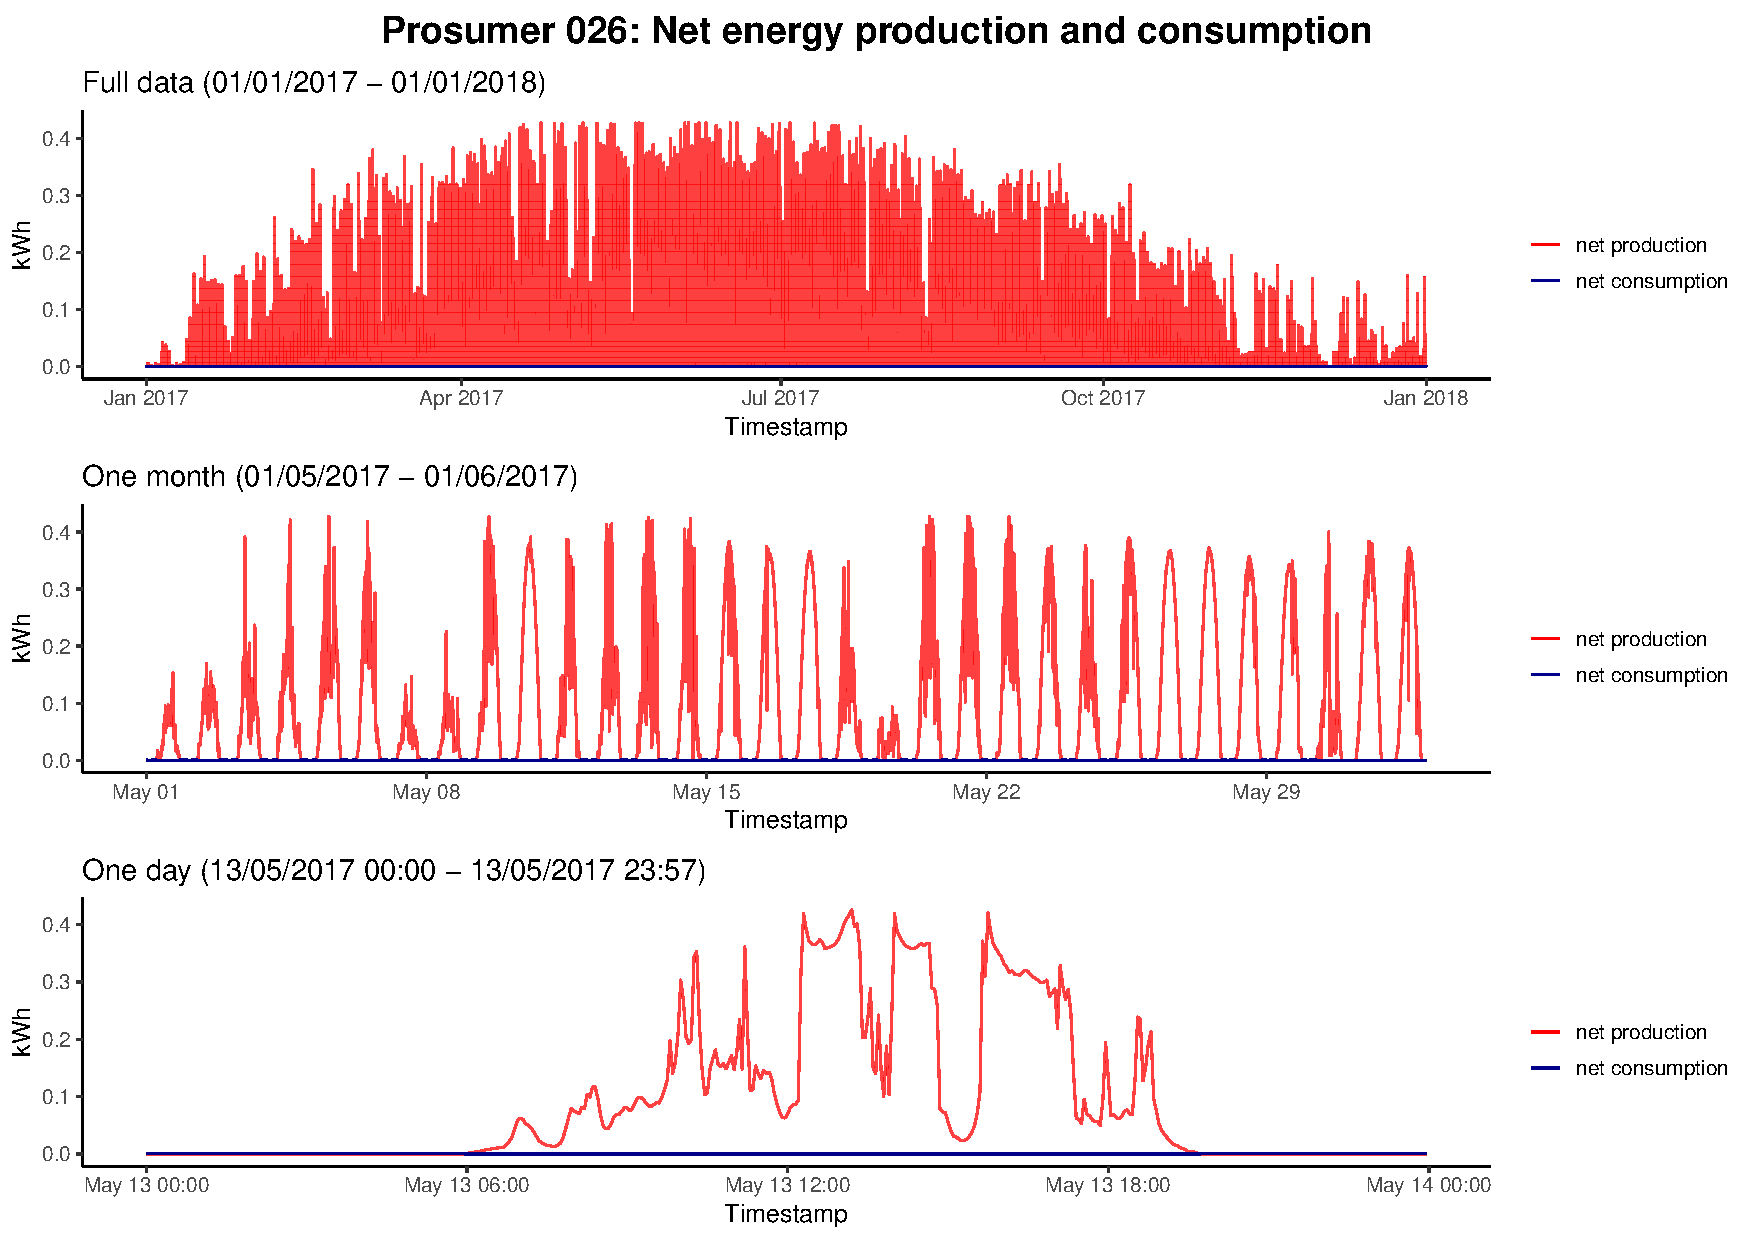
\includegraphics[width=\textwidth]{thesis/graphs/timeseries/p026_prod&cons.pdf}
\end{minipage}
\begin{minipage}[h]{\dimexpr.5\textheight-0.15em}
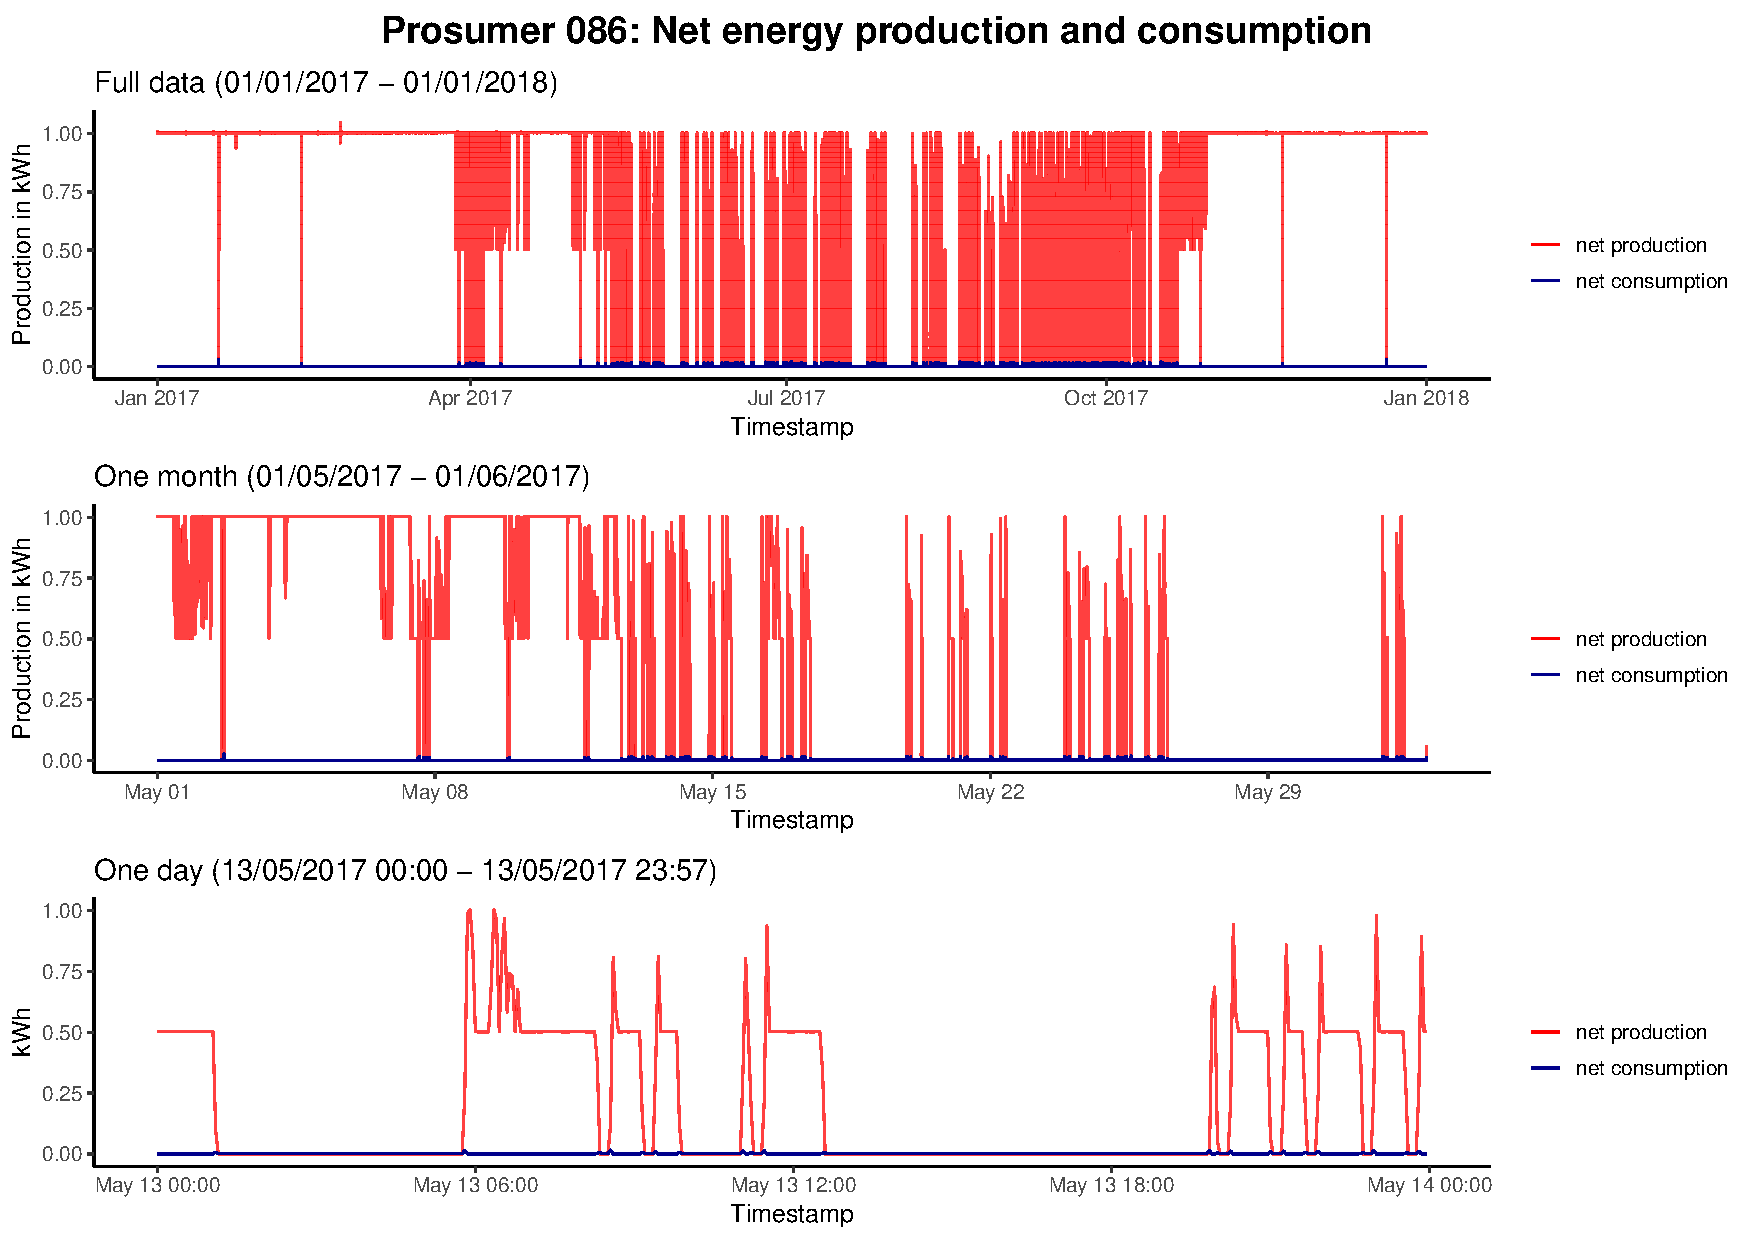
\includegraphics[width=\textwidth]{thesis/graphs/timeseries/p086_prod&cons.pdf}
\end{minipage}

\caption[Energy consumption and production recordings of prosumers 026 and 086]{Energy consumption and production recordings of prosumers 026 and 086. The first panel in the respective graph shows the full year 2017, the second panel zooms in to one month (May), and the third panel zooms in to one day (May, 13). \quantnet\href{https://github.com/QuantLet/BLEM/tree/master/BLEMplotEnergyData}{BLEMplotEnergyData}}
\label{Fig:energyconsprod_p026p086}

\end{sidewaysfigure}

In conclusion, it becomes clear that the prosumers' net energy consumption and production follow much less easily explained patterns. The net energy consumption is much more heterogeneous. Additionally, most prosumer data sets do not contain any recordings of net energy production at all. Of those prosumers that do have positive net production values, most surpass the energy consumption of a typical household with their net energy production by far. Implications of this for the suitability of the data sets for the prediction task at hand will be discussed in Section~\ref{Sec:Data;Subsec:Exclusion}.

%%%%%%%%%%%%%%%%%%%%%%%%%%%%%%%%%%%%%
%%%   Peculiarities in the data   %%%
%%%%%%%%%%%%%%%%%%%%%%%%%%%%%%%%%%%%%

\subsection{Peculiarities in the data}\label{Sec:Data;Subsec:Peculiarities}

%%%%%%%%%%%
\subsubsection{Consumer data sets}

The data sets were analyzed for peculiarities in the time series patterns that seemed to be systematically different than the majority of data sets. One such peculiarity is the occurrence of zero values. In any household that does not produce its own energy (pure consumer household), energy consumption of 0 kWh, even only for a very short period of time, seems to be very unlikely (apart from the rare case of a power outage in the area or when the main switch of the household is turned off). Thus, it is not surprising that 93~\% of the data sets do not contain any 0 kWh measurements per 3-minute interval at all. Of the remaining 6 data sets, one contains just a single measurement of 0 kWh, which seems plausible. The other data set with a negligible amount of zero values is consumer 082 which was discussed in detail in Section~\ref{Sec:Data;Subsec:Description}. In Figure~\ref{Fig:energycons_c082} showing consumer 082 consumption values, it is visible that although the consumption pattern does not change substantially, the lowest values of the daily fluctuations are lower in the second half of 2017 than in the first half. However, this seems still a plausible consumption pattern for a typical household. The other five data sets, on the contrary, contain between 34 and 54~\% of zero values. Examining the consumption time series more closely also reveals, that these households exhibit a systematically different consumption pattern that one would expect from a typical household.

\begin{sidewaysfigure}[htbp]
    \centering
    \begin{minipage}[ht]{\dimexpr.5\textheight-0.15em}
    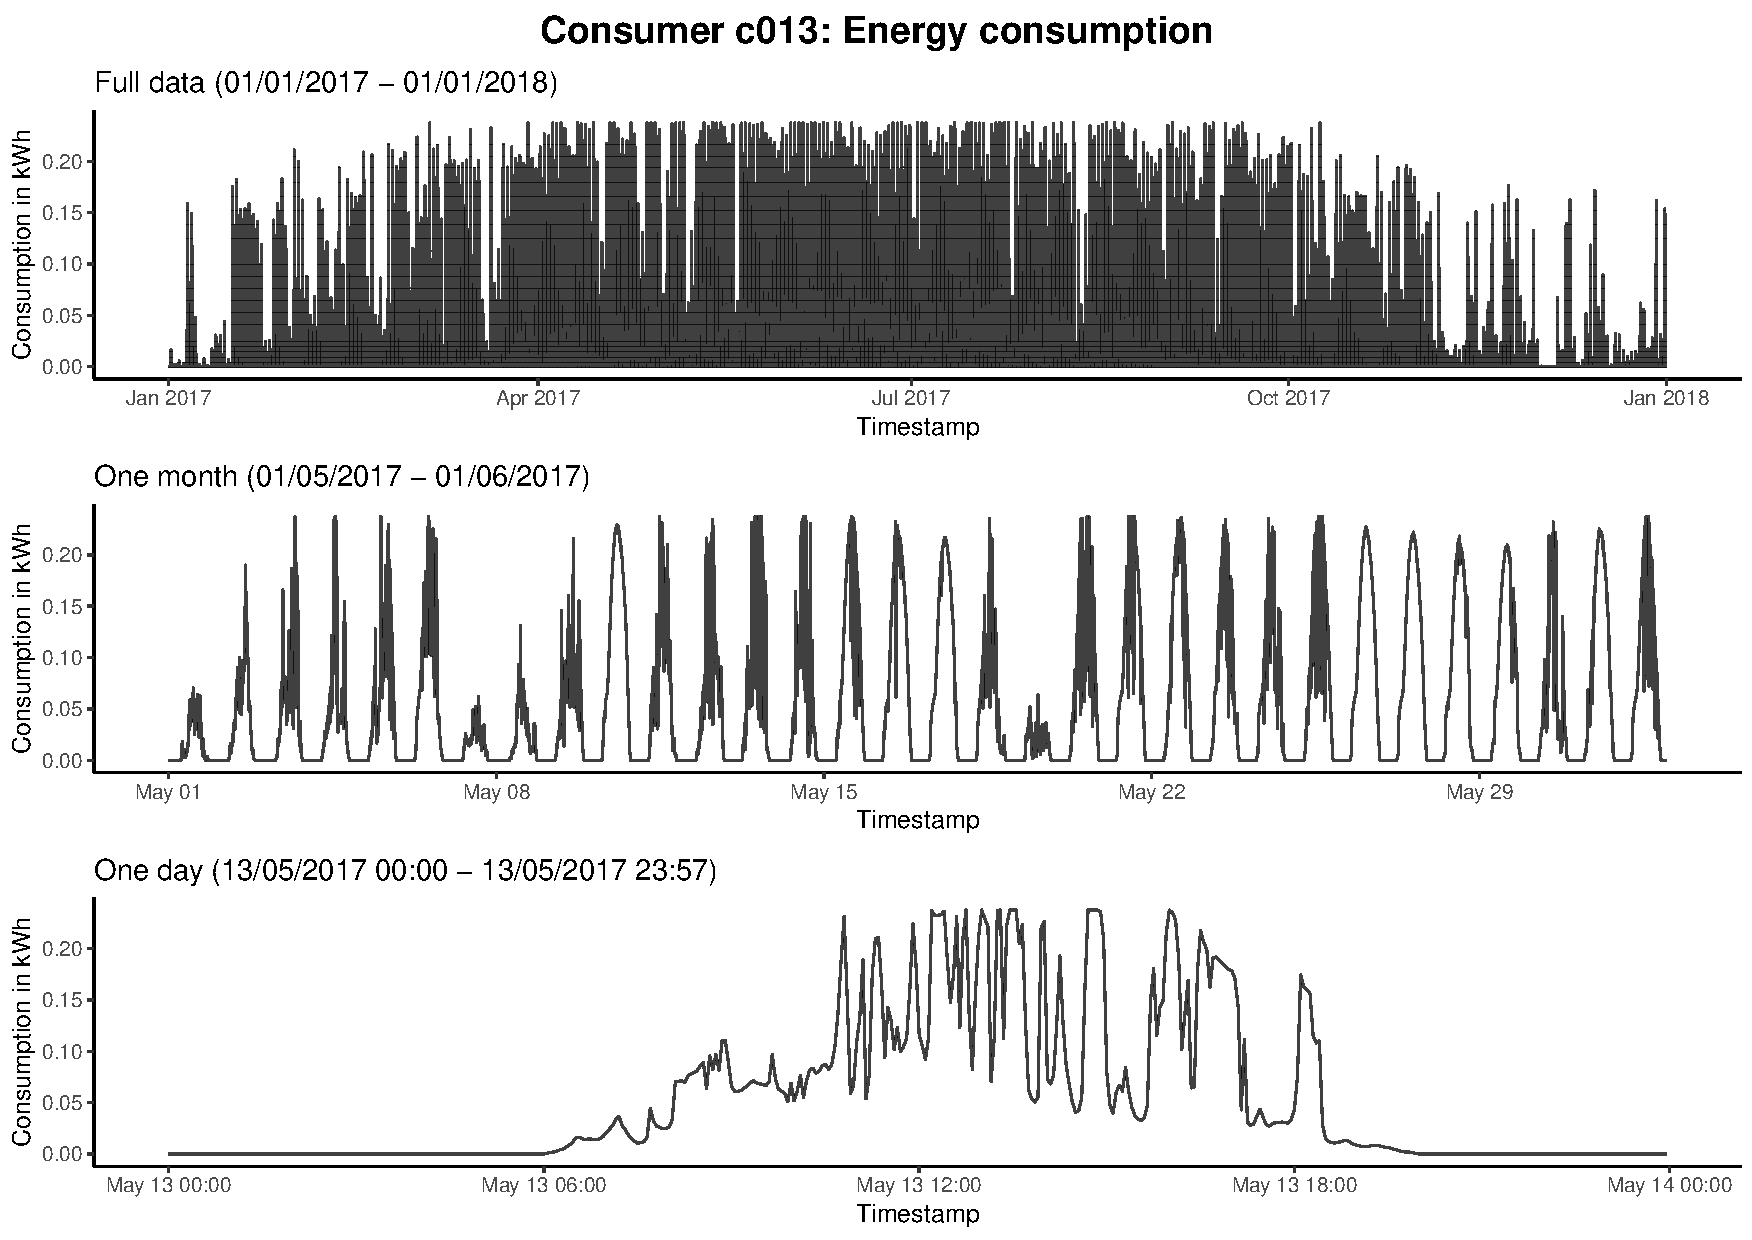
\includegraphics[width=\textwidth]{thesis/graphs/timeseries/c013_cons.pdf}
    \end{minipage}
    \begin{minipage}[ht]{\dimexpr.5\textheight-0.15em}
    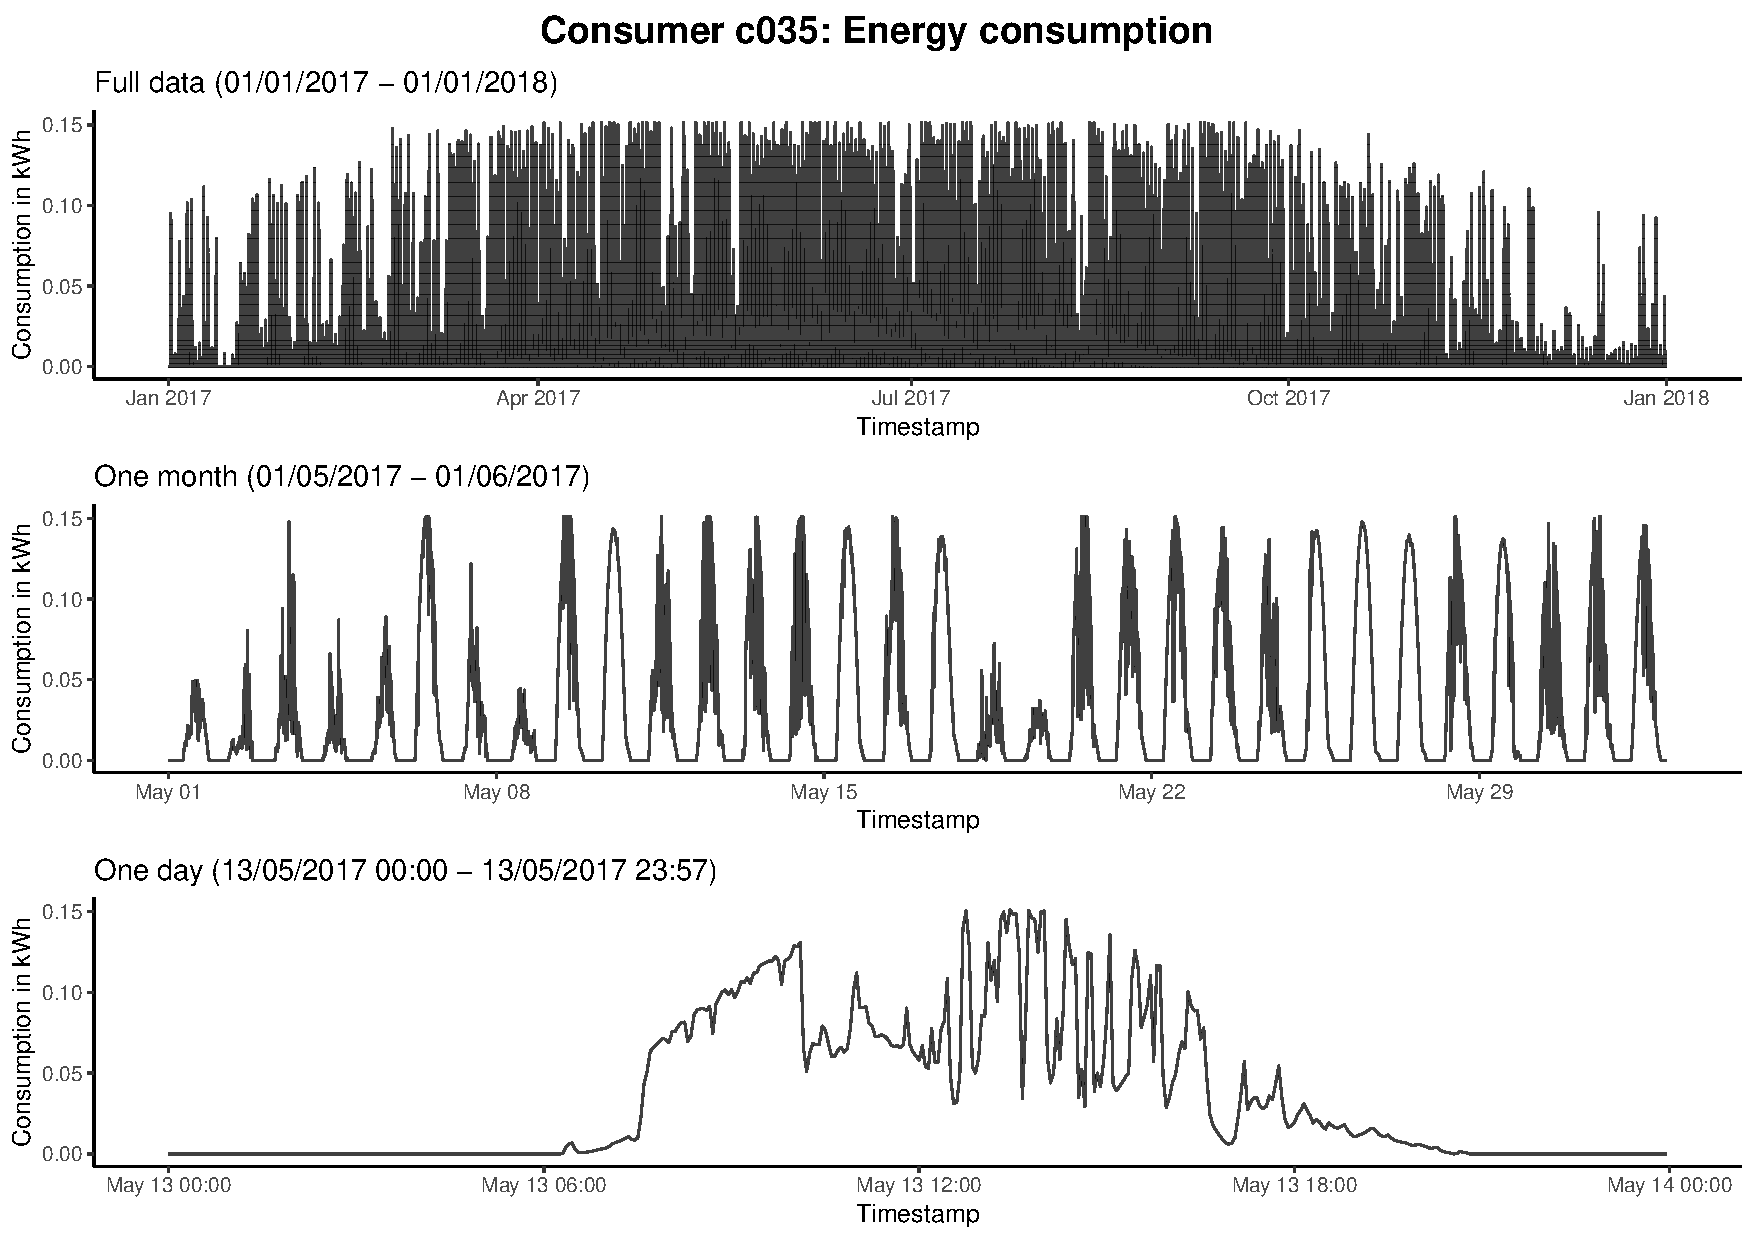
\includegraphics[width=\textwidth]{thesis/graphs/timeseries/c035_cons.pdf}
    \end{minipage}\\
    
    \begin{minipage}[ht]{\dimexpr.5\textheight-0.15em}
    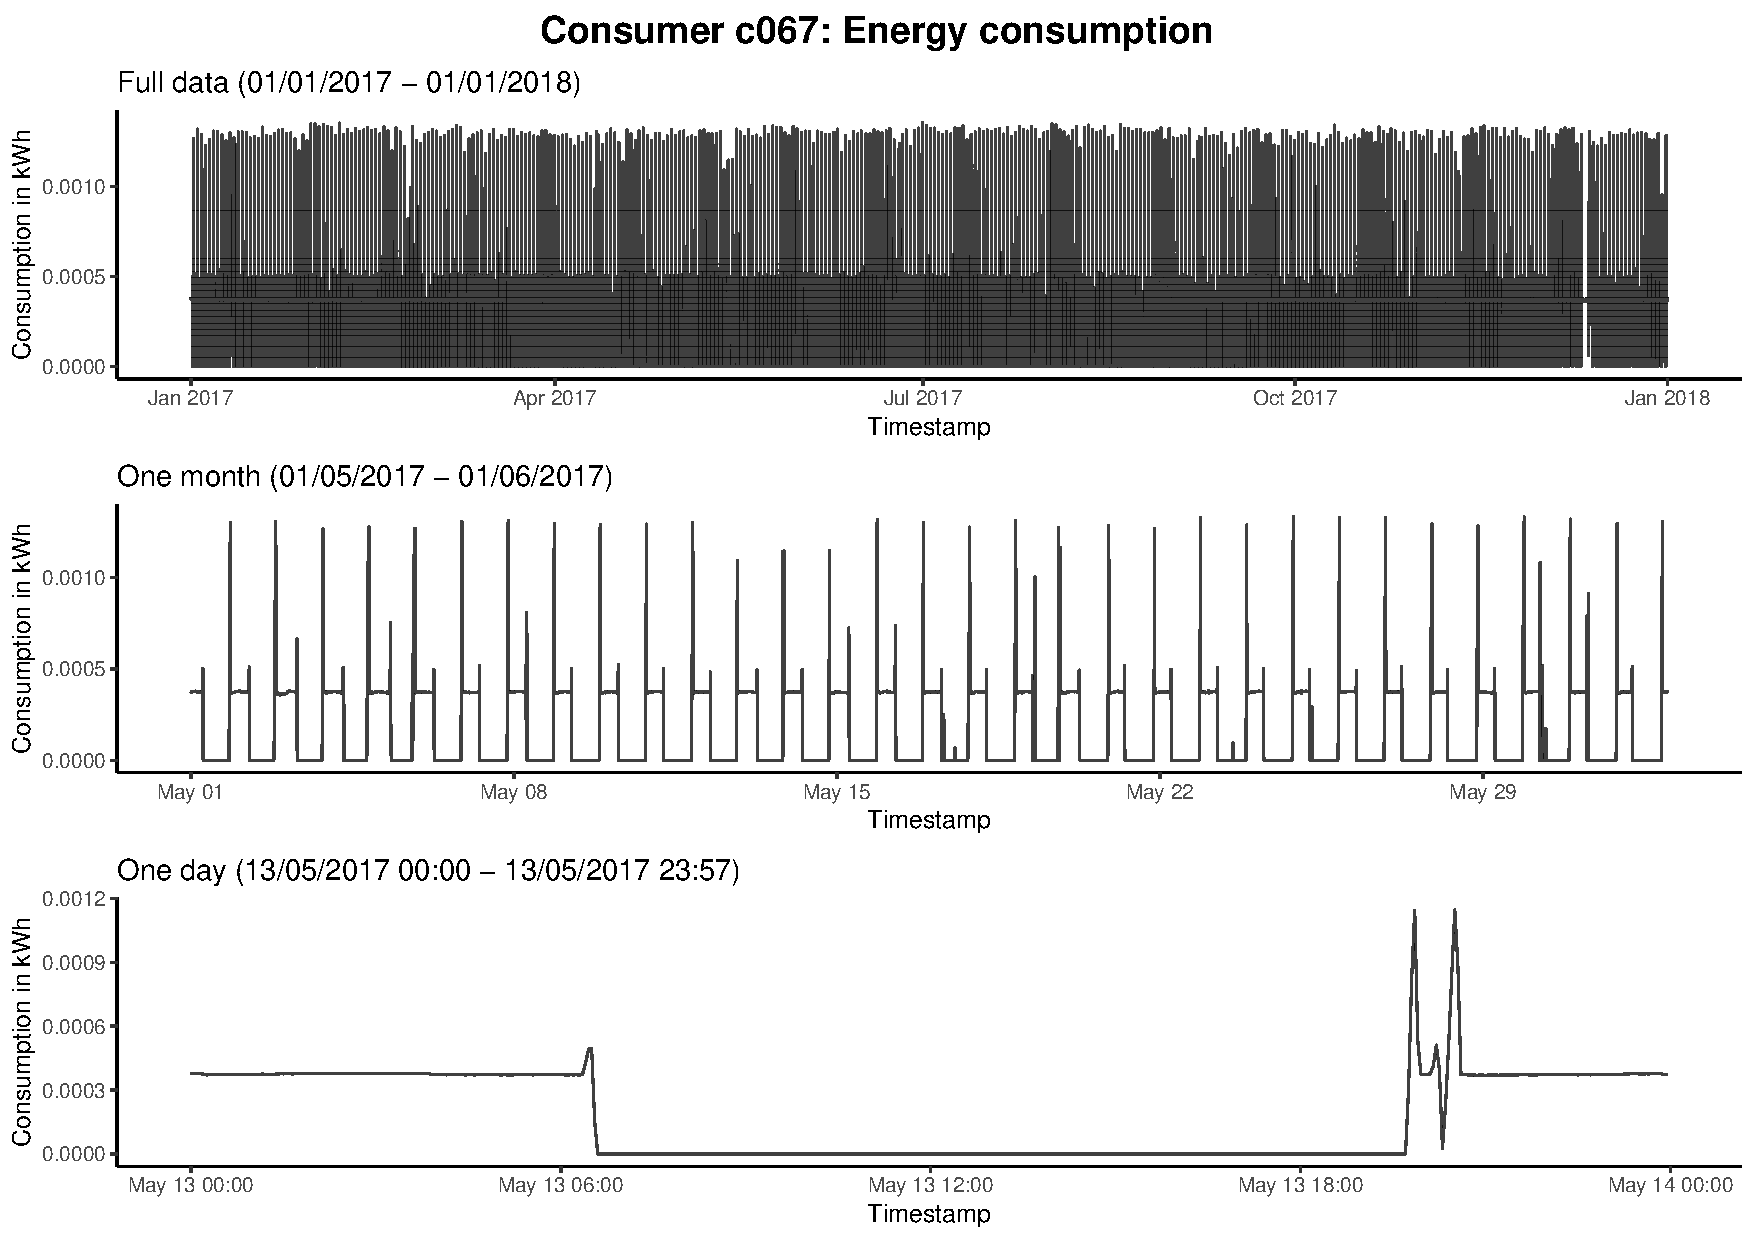
\includegraphics[width=\textwidth]{thesis/graphs/timeseries/c067_cons.pdf}
    \end{minipage}
    \begin{minipage}[ht]{\dimexpr.5\textheight-0.15em}
    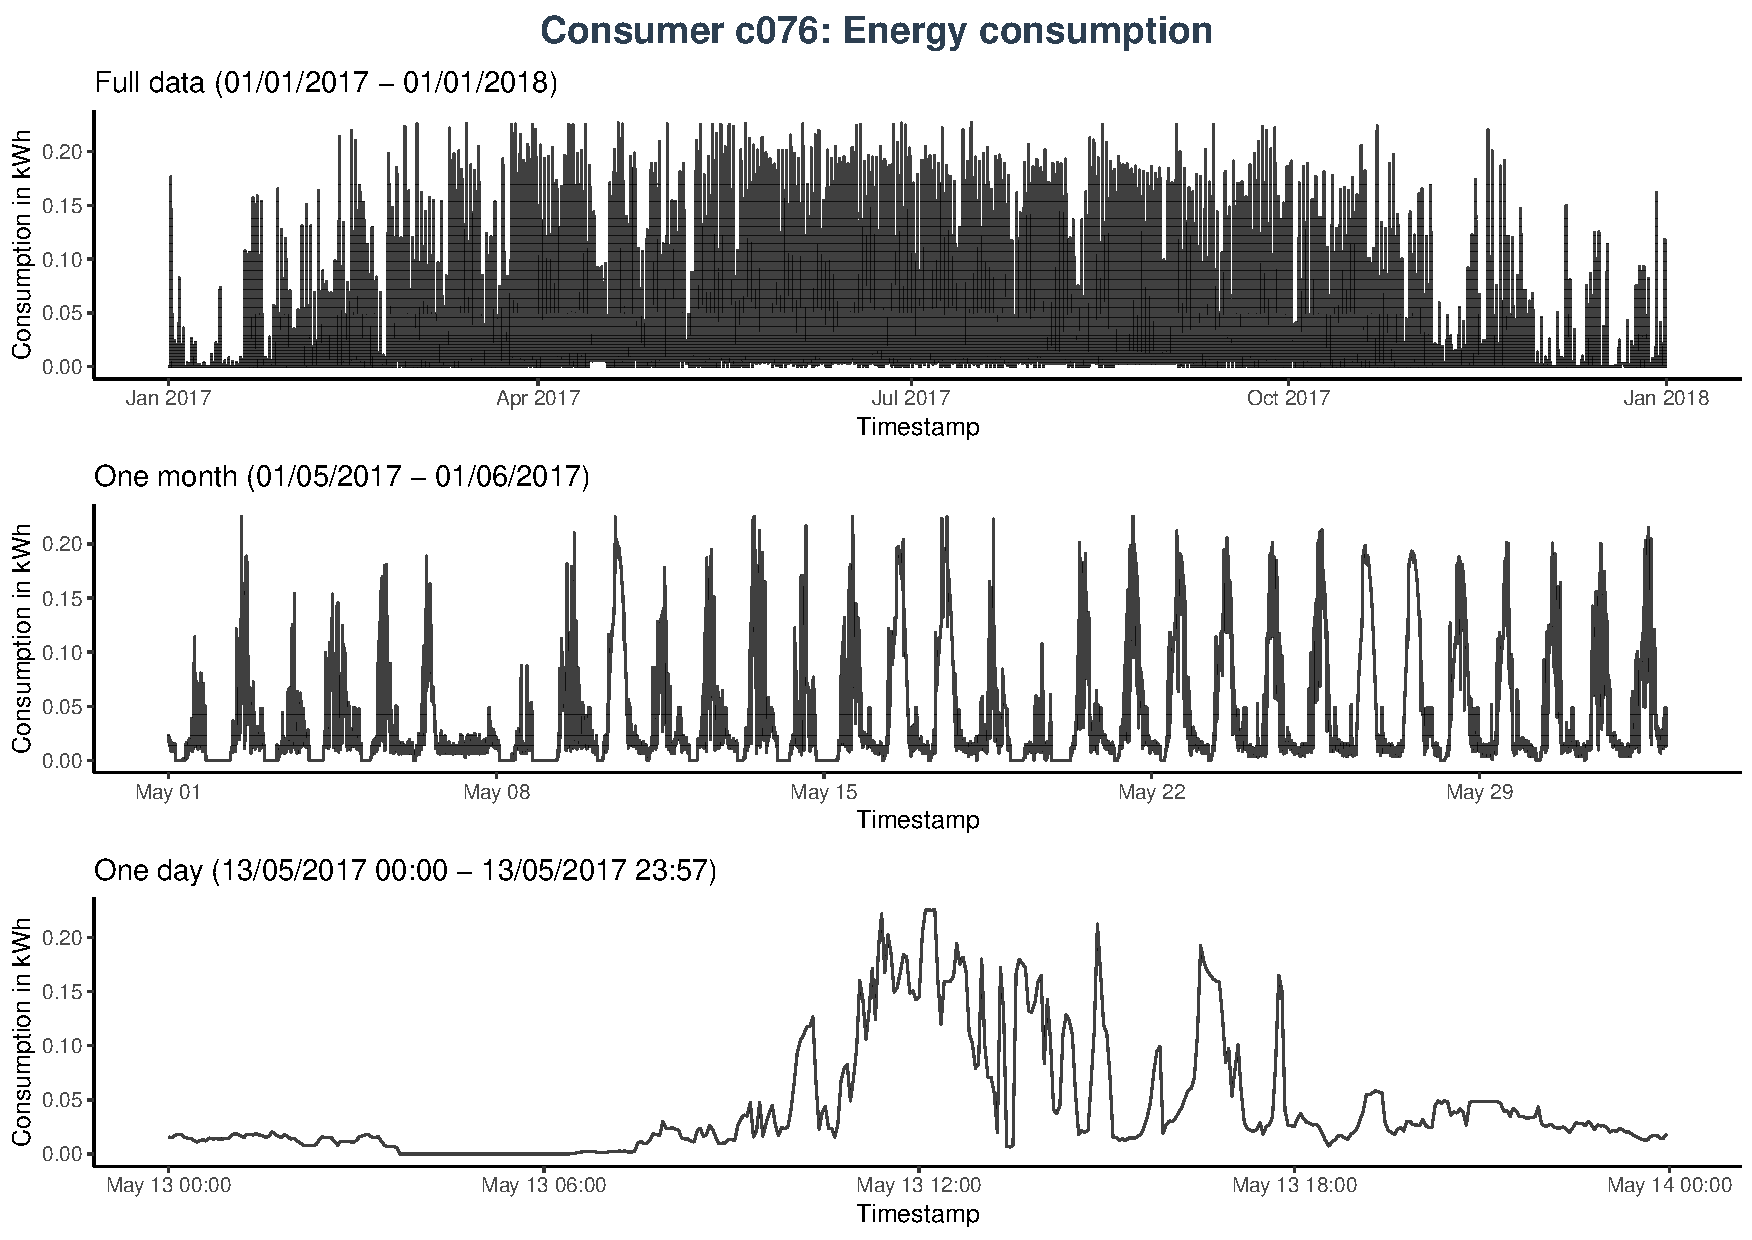
\includegraphics[width=\textwidth]{thesis/graphs/timeseries/c076_cons.pdf}
    \end{minipage}
    
    \caption[Energy consumption recordings of consumers with conspicuous consumption patterns]{Energy consumption recordings of consumers with conspicuous consumption patterns. \quantnet\href{https://github.com/QuantLet/BLEM/tree/master/BLEMplotEnergyData}{BLEMplotEnergyData}}
    \label{Fig:consenergycons_peculiar}
\end{sidewaysfigure}

Figure~\ref{Fig:consenergycons_peculiar} shows the time series of the aforementioned four consumers with a high share of zero measurements. Consumer 013 and 035 both show a very similar pattern of daily energy consumption. Looking at the middle panel of the two upper graphs in Figure~\ref{Fig:consenergycons_peculiar}, the regularity of the consumption increases and decreases for each day is striking. The lower panel shows again, exemplary, May 13. Energy consumption starts to (almost linearly) increase at about 6 a.m. and decreases to 0 kWh at about 6 p.m. This also explains the 52.77 and 54.02~\% of zero values in those to data sets: almost exactly 12 hours per day (from midnight to 6 a.m. and from 6 p.m. to midnight) the consumption is zero, while the energy consumption fluctuates in the meantime with a relatively high ``base" consumption. Switching back to the middle panel, it is noticeable that there are some days in May with an even smoother energy consumption increase and decrease over the course of the day. As there is no further socio-demographic data available, we can only guess what the reason for such different consumption patterns are. The most likely explanation seems to be, that the consumption time series of consumer 013 and 035 belongs to a small business rather than to a household.

The lower two graphs show the energy consumption time series of consumer 067 and consumer 076. Consumer 067 consumption pattern zoomed in to one month (middle panel) rather looks like an electrocardiogram than what one would expect from a household energy consumption time series. The regularity of amplitude and frequency is obvious but not easily explained. Consumers 076 consumption pattern looks less suspicious at first sight. However, closer inspection reveals the same daily pattern of increasing consumption throughout the day and very low to zero energy consumption at night. This again rather resembles the energy consumption pattern of a business building or office rooms.



%%%%%%%%%%%
\subsubsection{Prosumer data sets}

For prosumers, peculiarities in the time series pattern can be found either in the net energy consumption or net energy production or in combination. As net energy consumption is much more heterogeneous in the prosumer data sets than in the consumer data sets, it is less obvious what patterns fall outside the norm. However, some prosumer still exhibit obvious anomalies in their consumption patterns. Prosumer 046, 061, and 079 stand out as their consumption is zero for the largest part of the year. This would be an expected pattern if they were net energy producers during this time period. However, as they do not feed in any produced energy at all in 2017, this consumption pattern indicates a data problem. 
Prosumer 038 attracts attention by having a very low total net energy consumption of just 18.168 kWh in 2017 and zero net production. Moreover, this energy is consumed at an extremely low level of around 0.0001 kWh with a standard deviation of $\sigma=2\times10^{-6}$ and just one single drop from this level to zero in the whole year (see Figure~\ref{Fig:energycons_p038}). Six more prosumers exhibit a similar pattern of stable level of net energy consumption with occasional drops to zero but no spikes above this stable level. None of them is a net energy producer at any time.

\begin{figure}[htbp]
 \centering
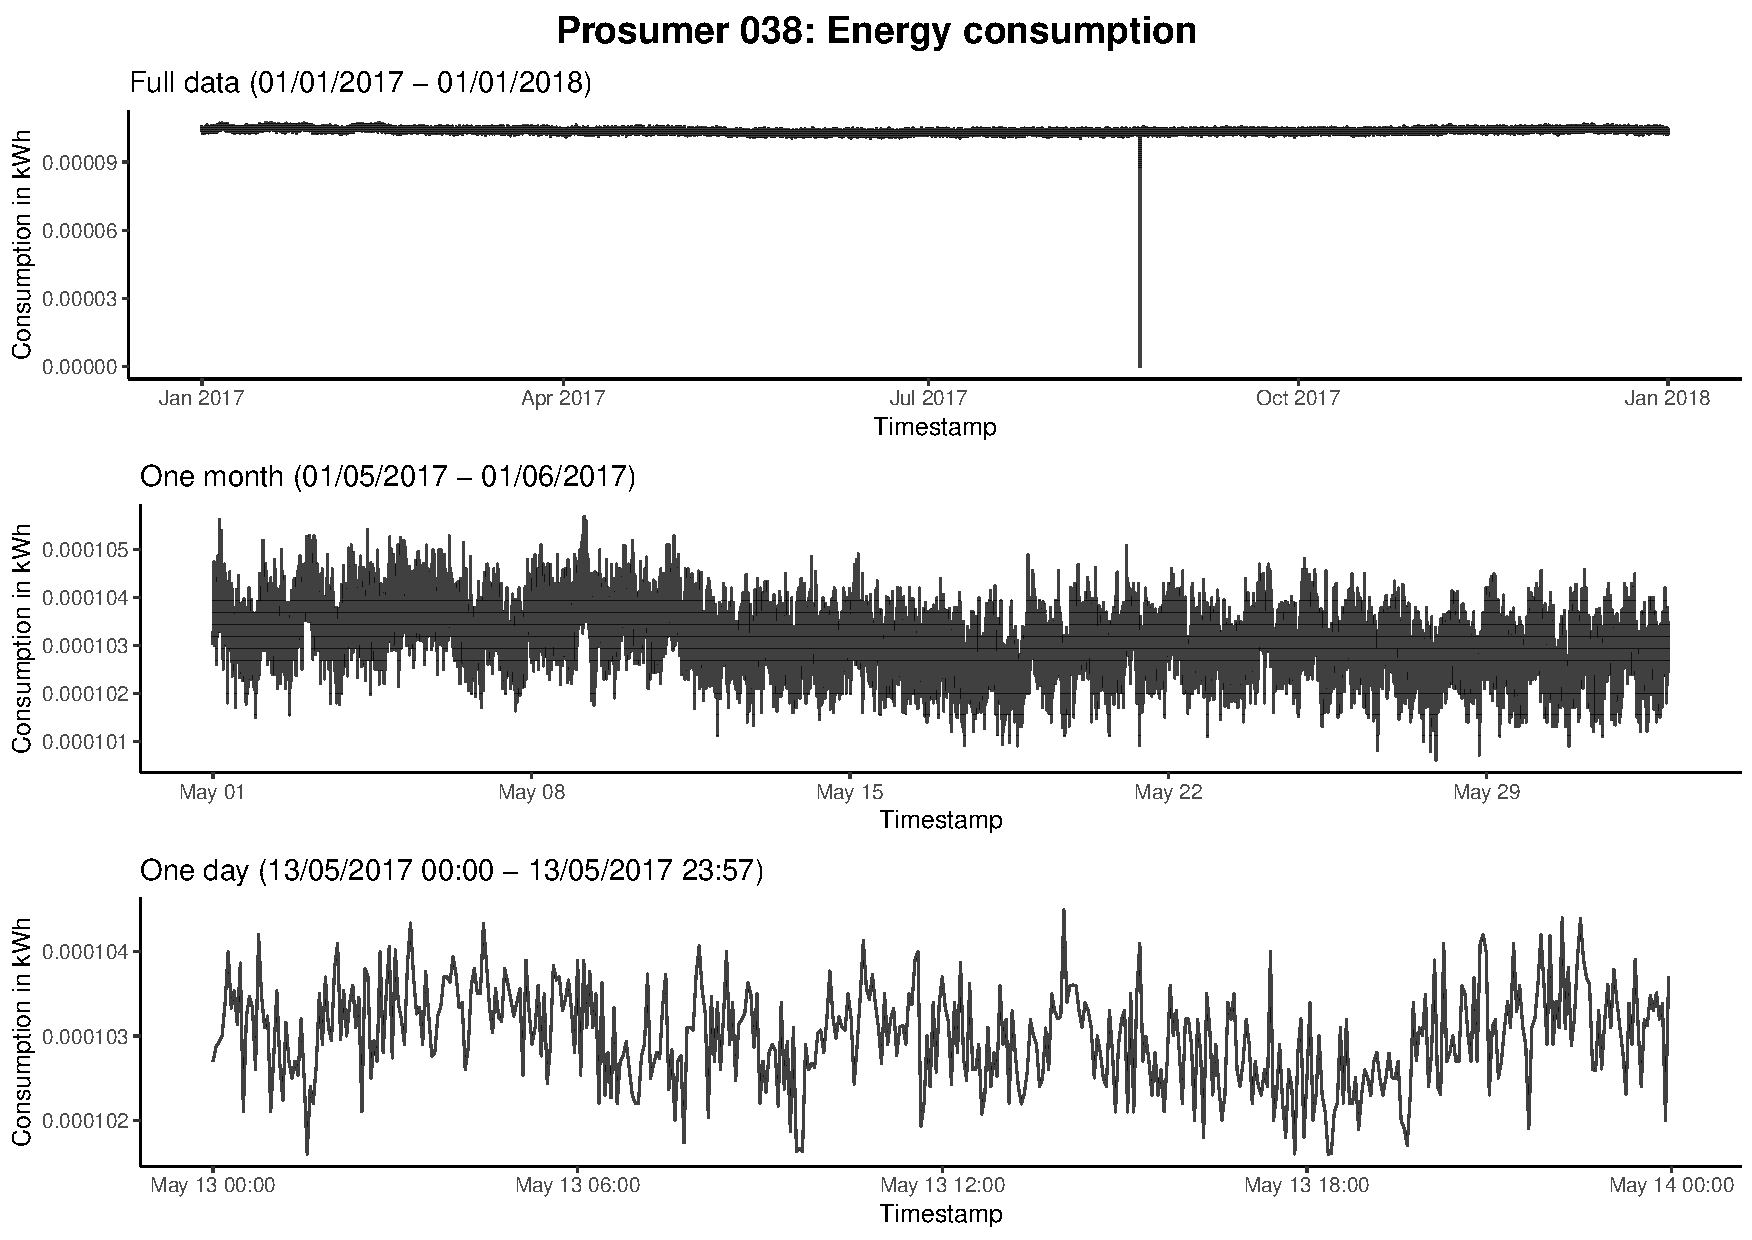
\includegraphics[width=\textwidth]{thesis/graphs/timeseries/p038_cons.pdf}
\caption[Energy consumption recordings of prosumer 038]{Energy consumption recordings of prosumer 038. The first panel shows the full year 2017, the second panel zooms in to one month (May), and the third panel zooms in to one day (May, 13). \quantnet\href{https://github.com/QuantLet/BLEM/tree/master/BLEMplotEnergyData}{BLEMplotEnergyData}}
\label{Fig:energycons_p038}
\end{figure}

Lastly, prosumer 019 is worth mentioning as it is the only prosumer data set that records a total net energy consumption of 0 kWh for 2017. As the net energy production, however, contains a substantial amount of zero values as well, it seems implausible that prosumer 019 is a regular household. For a household, it appears unlikely that the energy consumption is always zero when the energy production is zero as well.

Regarding the prosumer time series, most of the data sets are peculiar in so far as they have only zero net production values. It seems somewhat unlikely that any household equipped with energy production capacities consumes more than it produces over the whole course of the year at any point in time. However, it is unfortunately not possible to get feedback from Discovergy due to privacy and internal policy reasons on why 84 out of 100 prosumer data sets do not record any energy fed into the grid at all.

Of the remaining 14 data sets, prosumer 084 and 085 stand out as their net energy production time series is almost a flat line at 2.5 kWh per 3-minute interval. Their graphs are shown in Figure~\ref{Fig:energyconsprod_p084p085}.

\begin{sidewaysfigure}[htbp]
\centering
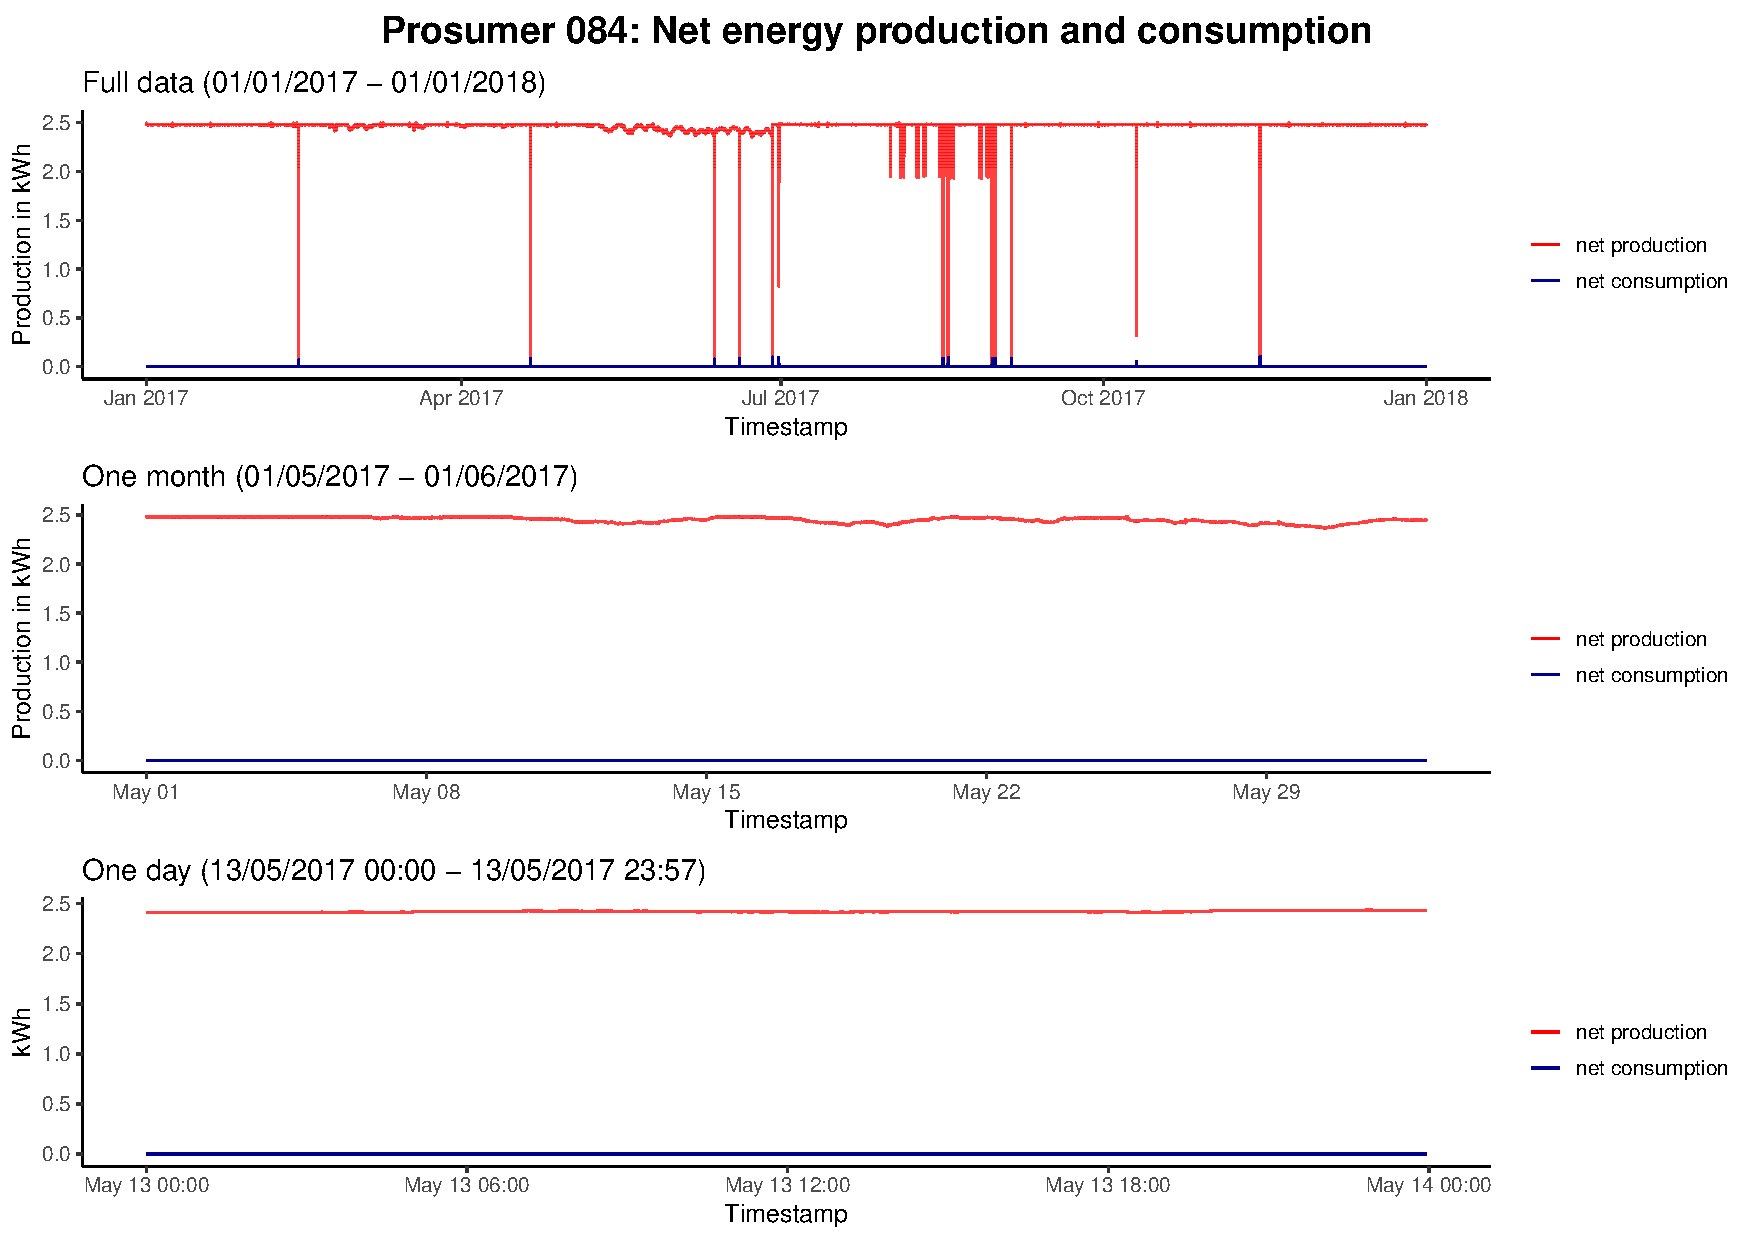
\includegraphics[width=.5\textwidth-0.15em]{thesis/graphs/timeseries/p084_prod&cons.pdf}
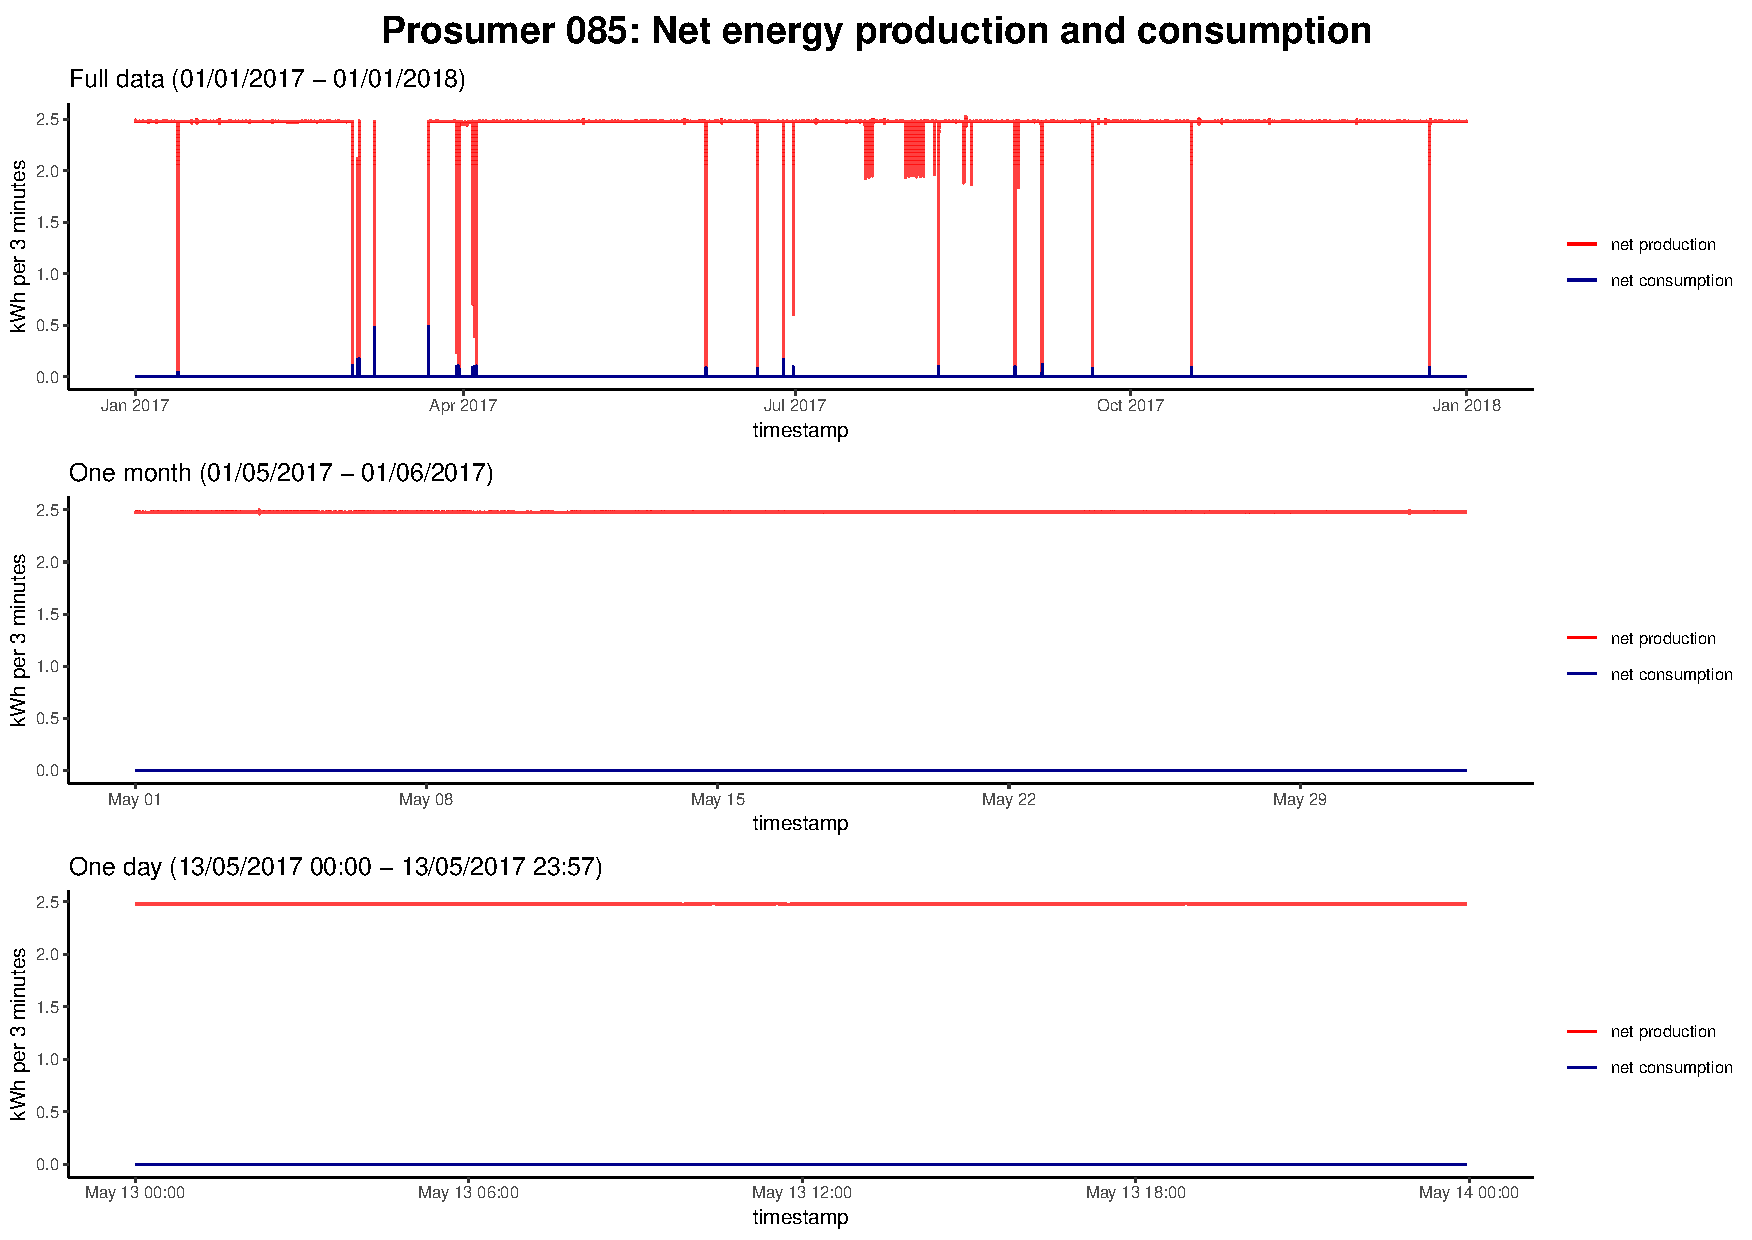
\includegraphics[width=.5\textwidth-0.15em]{thesis/graphs/timeseries/p085_prod&cons.pdf}

\caption[Energy consumption and production recordings of prosumers 084 and 085]{Energy consumption and production recordings of prosumers 024 and 085. The first panel in the respective graph shows the full year 2017, the second panel zooms in to one month (May), and the third panel zooms in to one day (May, 13). \quantnet\href{https://github.com/QuantLet/BLEM/tree/master/BLEMplotEnergyData}{BLEMplotEnergyData}}
\label{Fig:energyconsprod_p084p085}
\end{sidewaysfigure}

In conclusion, it seems like the majority of prosumer data sets with non-zero net production values were recorded by smart meters that just record the energy production of a certain installation and not of a household with production capacity. This is not per se a problem, as these installations can act as a individual agent on a local energy market. Even though, they might belong to a household with a separate smart meter, they can sell energy through their own smart meter while the related household's smart meter buys energy. If both smart meters are connected to the same blockchain wallet, this automatically solves the challenge of pricing the energy relative to the own consumption.

%%%%%%%%%%%%%%%%%%%%%%%%%%%%%%
%%%   Data sets excluded   %%%
%%%%%%%%%%%%%%%%%%%%%%%%%%%%%%

\subsection{Data sets excluded}\label{Sec:Data;Subsec:Exclusion}
The data sets of consumer 013, 035, 067 and 076 shown in Figure~\ref{Fig:consenergycons_peculiar} where excluded from the prediction task for the reasons discussed in Section~\ref{Sec:Data;Subsec:Peculiarities}. These four consumers plus one additional (consumer 082) exhibited large shares of zero consumption values. Further, consumer 046 was excluded as the consumption time series was flat for the most part of 2017. After some initial fluctuations in the first quarter, all fluctuations stopped entirely. Four more consumers were excluded due to conspicuous regularity in daily or weekly consumption patterns. Lastly, consumer 080 was excluded due to very low and stable consumption values with very rare, extreme spikes. The time series graphs of all additionally to the ones shown in Figure~\ref{Fig:consenergycons_peculiar} excluded consumer data sets are shown in Appendix~\hyperlink{AppA1:Figures:Excludedc}{A1}. Consumer 026 was excluded not due to peculiarities in the consumption patterns but due to missing data. For some unknown reason, the last recorded measurement for consumer 026 is 2017-12-29 07:03:00. As the inclusion of this shorter time series would lead to difficulties in the forecasting algorithms, this data set was excluded as well.

Out of the 100 prosumer data sets, 86 were excluded from the prediction task due to zero total net energy production in 2017. These ``prosumers" would not act as prosumers in a local energy market as they never actually supply a production surplus to the market. Moreover, as their net energy production is always zero, their net energy production shows no variation which is a necessary precondition to train any prediction model.

Of the remaining 14 prosumer data sets, prosumer 012 was excluded as the total net energy it fed into the grid in 2017 was just 22.144 kWh. Even though, the feed in occurred continuously over the whole year, it was never exceeded 0.0013 kWh per 3-minute interval with a mean of 0.0001 kWh, which is too small to be of interest. Prosumer 015 was excluded as it only fed energy into the grid in the period from 06.01.2017 to 19.01.2017. For all other measurement points the net energy production was zero. The time series graph of the two excluded prosumer data sets with production data are shown in Appendix~\hyperlink{AppA2:Figures:Excludedp}{A2}

Hence, 88 consumer and 12 prosumer data sets remained for the prediction tasks. All data sets included a time stamp and the consumption time series for consumers respectively the production time series for prosumers with a total of 175,200 data points each.


%%%%%%%%%%%%%%%%%%%%%%%%%%%%%%%%%%%%%%%%%%%%%%%%%%%%%%%%%%%%%%%%%